
\section{Benchmark CG}
\subsection{Wyniki benchmarków - platforma ARM64}

\begin{figure}[H]
    \centering
    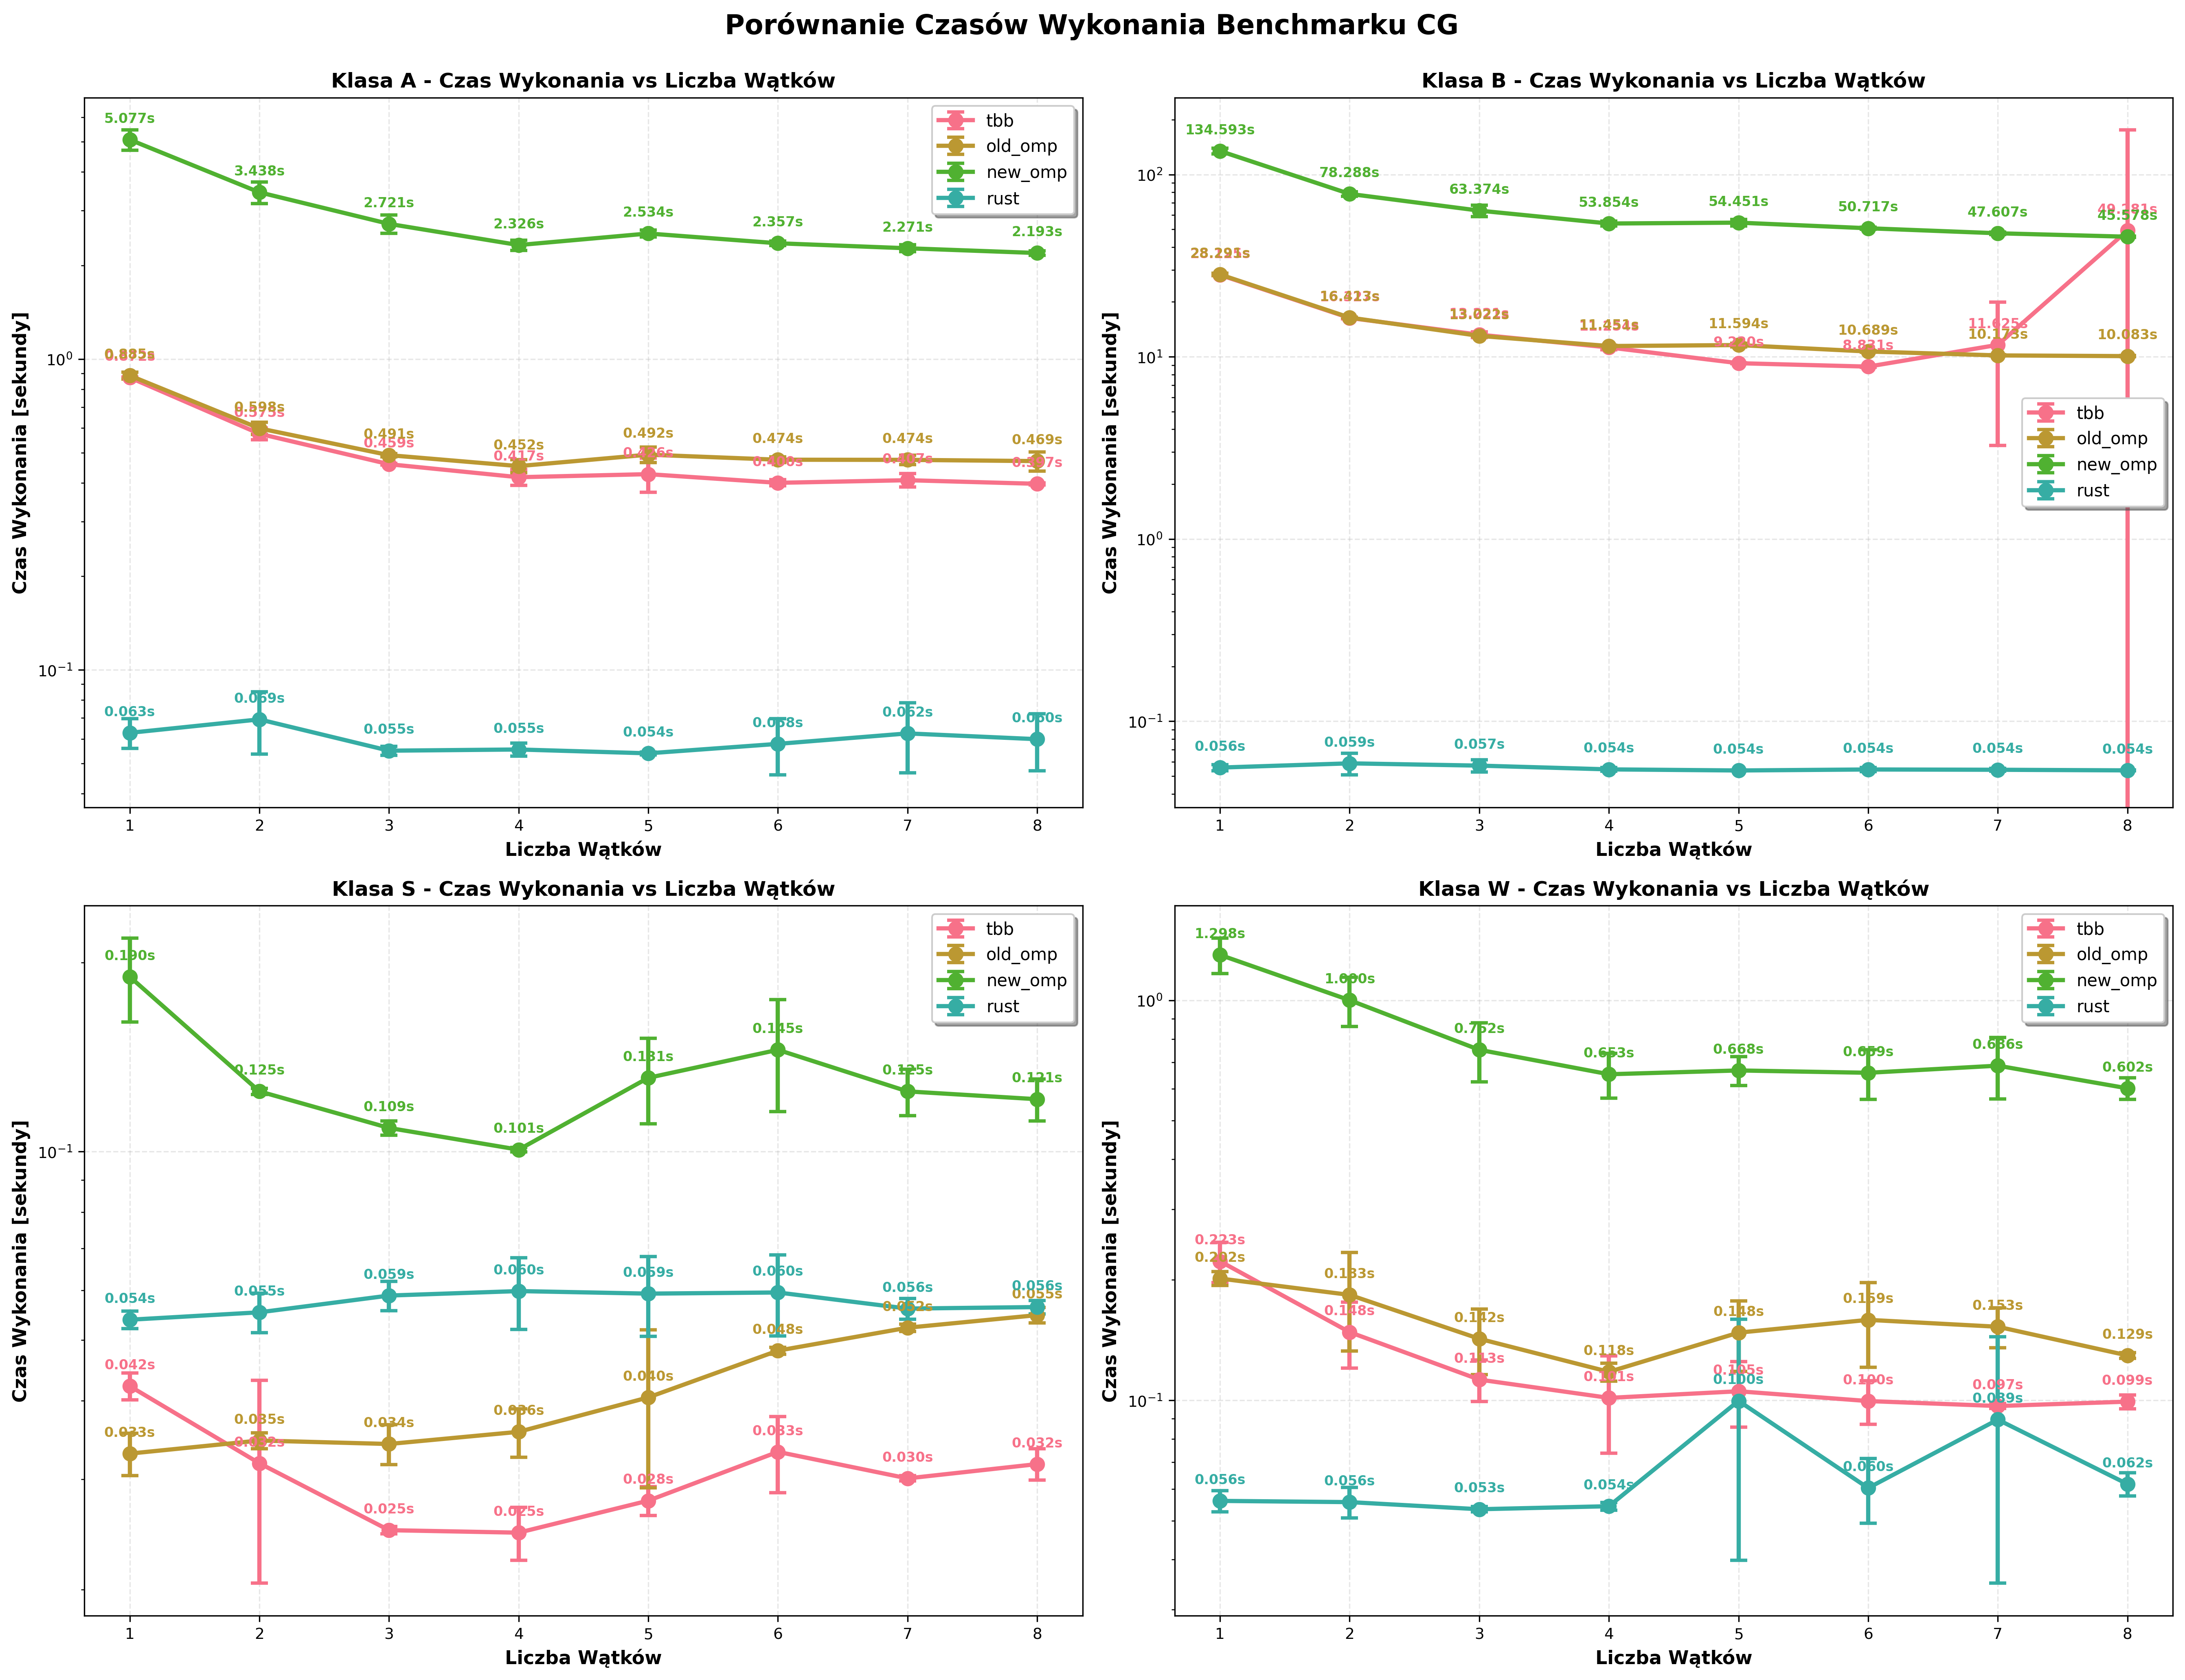
\includegraphics[width=\textwidth]{analiza/images/parallel/cg/cg_porownanie_czasow_wykonania.png}
    \caption{Porównanie czasów wykonania benchmarku CG dla klas S, W, A, B względem liczby użytych wątków}
    \label{cg_porownanie_czasow_wykonania}
\end{figure}

Na rysunku \ref{cg_porownanie_czasow_wykonania} zaprezentowano zestawienie czasów wykonania benchmarku CG dla czterech klas problemu: S, W, A oraz B, przy użyciu czterech różnych implementacji równoległości: TBB, OpenMP w wersji oryginalnej w stylu języka Fortran (old\_omp), OpenMP w wersji nowszej (new\_omp) oraz implementacji w języku Rust. Dla każdej z klas przedstawiono zależność czasu wykonania od liczby wątków (od 1 do 8). Wartości zostały zaprezentowane w skali logarytmicznej.

\begin{figure}[H]
    \centering
    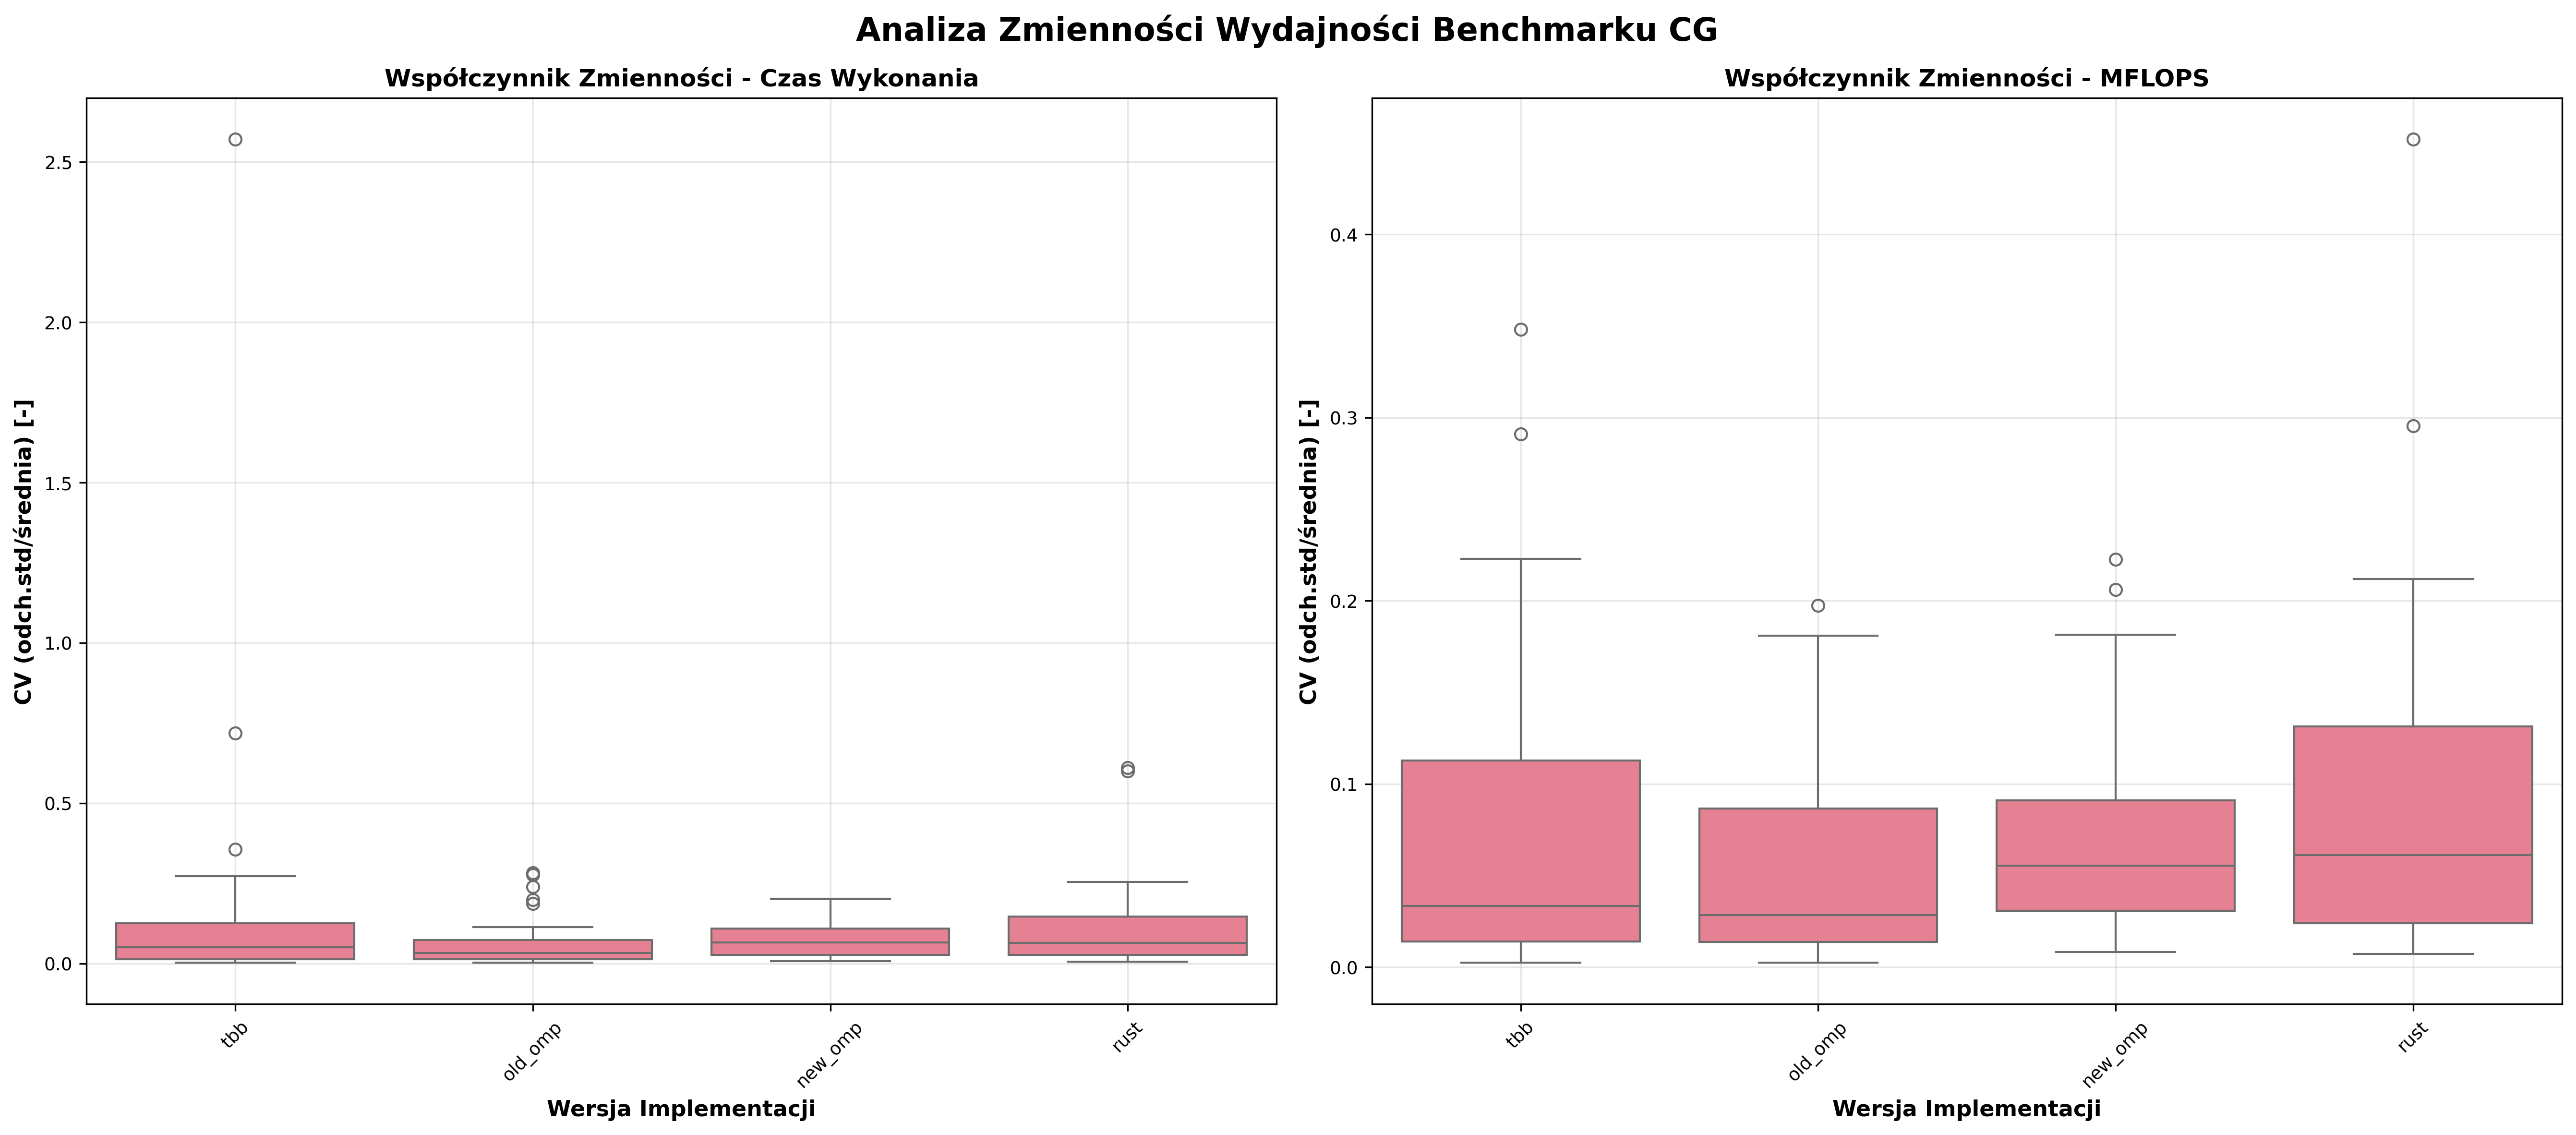
\includegraphics[width=\textwidth]{analiza/images/parallel/cg/cg_analiza_zmiennosci.png}
    \caption{Analiza zmienności czasów wykonania benchmarku CG dla klas S, W, A, B względem liczby użytych wątków}
    \label{cg_analiza_zmiennosci}
\end{figure}
Powyższy wykres - rysunek \ref{cg_analiza_zmiennosci} pudełkowy prezentuje współczynnik zmienności \eng{CV - coefficient of variation}, obliczony jako stosunek odchylenia standardowego do wartości średniej, w odniesieniu do czasu wykonania (lewy wykres) oraz uzyskiwanej wydajności (prawy wykres) dla różnych wersji implementacji benchmarku.

\subsubsection{Współczynnik Zmienności - Czas Wykonania}
Na lewym wykresie ukazano zmienność czasów wykonania dla każdej z implementacji:
\begin{itemize}
    \item old\_omp charakteryzuje się najniższą medianą współczynnika zmienności oraz małym rozrzutem danych, co świadczy o dużej stabilności czasów wykonania.
    \item new\_omp i rust wykazują porównywalną medianę, jednak większe rozproszenie wyników oraz obecność wartości odstających (outliers), co wskazuje na mniejszą deterministyczność wykonania.
    \item TBB mimo wysokiej wydajności (z poprzedniego wykresu) cechuje się największą zmiennością czasów wykonania, w tym także obecnością ekstremalnych wartości odstających, z których jedna przekracza wartość CV = 2.5. Może to wynikać z dynamicznego planowania zadań lub większego wpływu czynników systemowych.
\end{itemize}

\subsubsection{Współczynnik Zmienności - MFLOPS}
Na prawym wykresie przedstawiono zmienność osiąganej wydajności (MFLOPS):
\begin{itemize}
    \item old\_omp ponownie wypada najkorzystniej - niska mediana i mały rozrzut wartości świadczą o przewidywalnej wydajności obliczeniowej.
    \item new\_omp oraz TBB uzyskują nieco wyższe wartości CV, jednak nadal w akceptowalnym zakresie dla zastosowań równoległych.
    \item Rust wykazuje największą zmienność - mediany są wyższe, a pudełka wykresów (IQR) znacznie szersze. Sugeruje to brak spójności pomiędzy kolejnymi uruchomieniami, co może być efektem niedojrzałości środowiska wykonawczego lub specyfiki kompilatora.
\end{itemize}

\subsubsection{Klasa S}
Dla najmniejszej klasy problemu (S):
\begin{itemize}
    \item TBB osiąga najniższy czas wykonania (~0.025s przy 4 wątkach), lecz przy wyższych liczbach wątków nie obserwuje się dalszego przyspieszenia, a wręcz lekkie pogorszenie wyników.
    \item old\_omp i new\_omp zachowują się podobnie - czasy oscylują wokół 0.05s, bez wyraźnych korzyści z użycia więcej niż 3-4 wątków.
    \item Rust prezentuje najwyższe czasy dla tej klasy, co może wynikać z narzutu związanego z wielowątkowością przy małym rozmiarze danych - czasy są stabilne, ale wyraźnie wyższe (ok. 0.1s).
\end{itemize}

\subsubsection{Klasa W}
W klasie W obserwuje się interesujące różnice w zachowaniu implementacji:
\begin{itemize}
    \item Rust początkowo uzyskuje dobre wyniki, lecz występują duże odchylenia standardowe (szczególnie dla 6 wątków), co może sugerować problemy z równomiernym rozłożeniem obciążenia.
    \item TBB oraz old\_omp osiągają najlepsze czasy wykonania, ustabilizowane na poziomie około 0.1s przy większej liczbie wątków.
    \item new\_omp uzyskuje wyniki ponad 6 razy gorsze (0.6s), choć wykazuje stabilność i poprawę przy wzroście liczby wątków.
    \item Istotne jest także zauważenie, że dla tej klasy wszystkie implementacje poza Rustem wykazują wzorcową skalowalność, osiągając najniższe wartości przy najwyższej liczbie wątków.
\end{itemize}


\subsubsection{Klasa A}
Dla klasy A obserwujemy wyraźną poprawę czasu wykonania w przypadku wszystkich implementacji wraz ze wzrostem liczby wątków, jednak efektywność skalowania różni się w zależności od technologii:
\begin{itemize}
    \item Rust osiąga najniższe czasy wykonania, utrzymując się na poziomie ~0.05s już od 3 wątków, z minimalnymi wahaniami.
    \item TBB, old\_omp oraz new\_omp wykazują zbliżoną wydajność, stabilizując się wokół 0.47s od 5 wątków wzwyż.
    \item Implementacja new\_omp jako jedyna spośród implementacji C/C++ pokazuje znaczące różnice w czasie przy niższych liczbach wątków (1-3), jednak dalsze zwiększanie liczby wątków przynosi jedynie marginalne korzyści.
\end{itemize}

\subsubsection{Klasa B}
W przypadku klasy B występują znacznie większe czasy wykonania, co wynika z większej skali problemu:
\begin{itemize}
    \item Rust pozostaje niezmiennie na poziomie ~0.05s, co sugeruje potencjalnie nieprawidłowe wykonanie lub użycie sztucznie uproszczonej wersji benchmarku dla tej klasy.
    \item old\_omp i new\_omp wykazują wyraźną poprawę do około 10s przy 6-8 wątkach, przy czym new\_omp cechuje się nieco lepszą skalowalnością.
    \item TBB również osiąga podobny poziom wydajności jak OpenMP, ale obserwowana wartość dla 8 wątków wykazuje znaczące odchylenie standardowe, co może wskazywać na niestabilność działania w tej konfiguracji.
    \item Implementacja new\_omp nie przekracza 50 sekund od 6 wątków wzwyż, co pokazuje jej względną efektywność, mimo wyraźnie wyższych czasów bazowych.
\end{itemize}

%------------------------------

\begin{figure}[H]
    \centering
    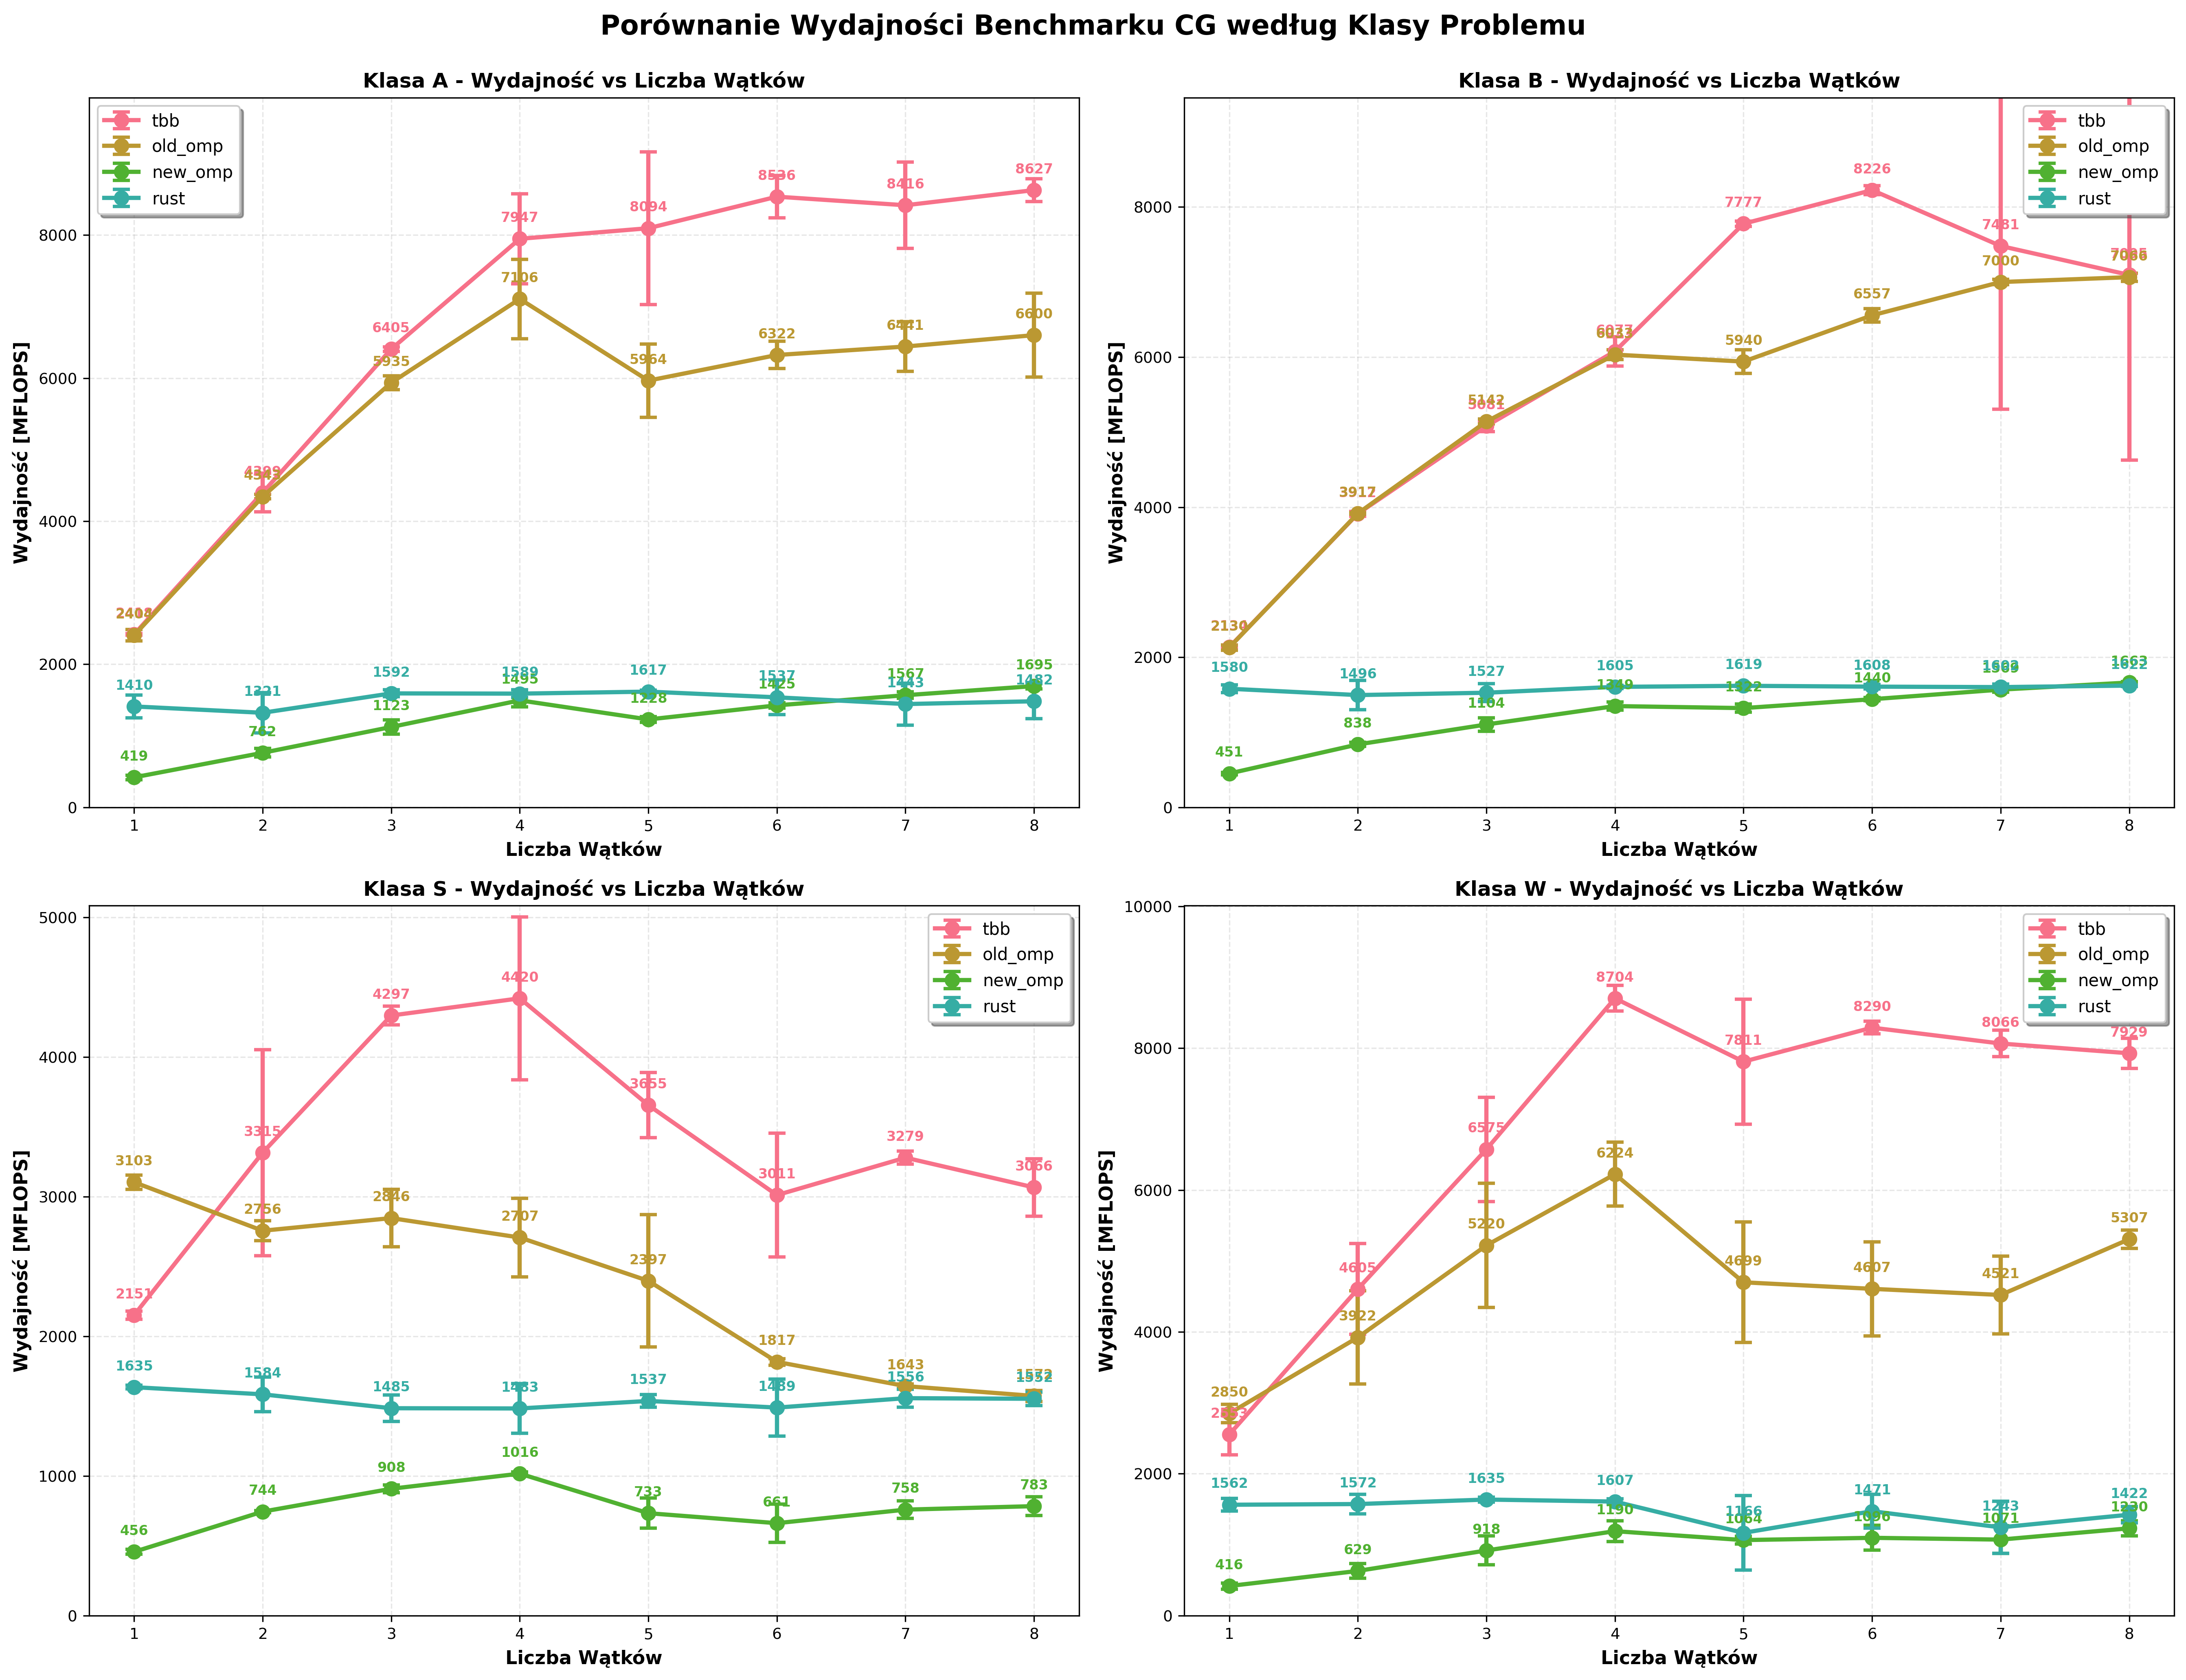
\includegraphics[width=\textwidth]{analiza/images/parallel/cg/cg_porownanie_wydajnosci.png}
    \caption{Porównanie wydajności benchmarku CG dla klas S, W, A, B względem liczby użytych wątków}
    \label{cg_porownanie_wydajnosci}
\end{figure}
Na wykresach na rysunku \ref{cg_porownanie_wydajnosci} zaprezentowano porównanie wydajności benchmarku CG mierzonej w MFLOPS (milionach operacji zmiennoprzecinkowych na sekundę). Wydajność została przedstawiona jako funkcja liczby wątków (1-8) dla czterech implementacji równoległych.

\begin{figure}[H]
    \centering
    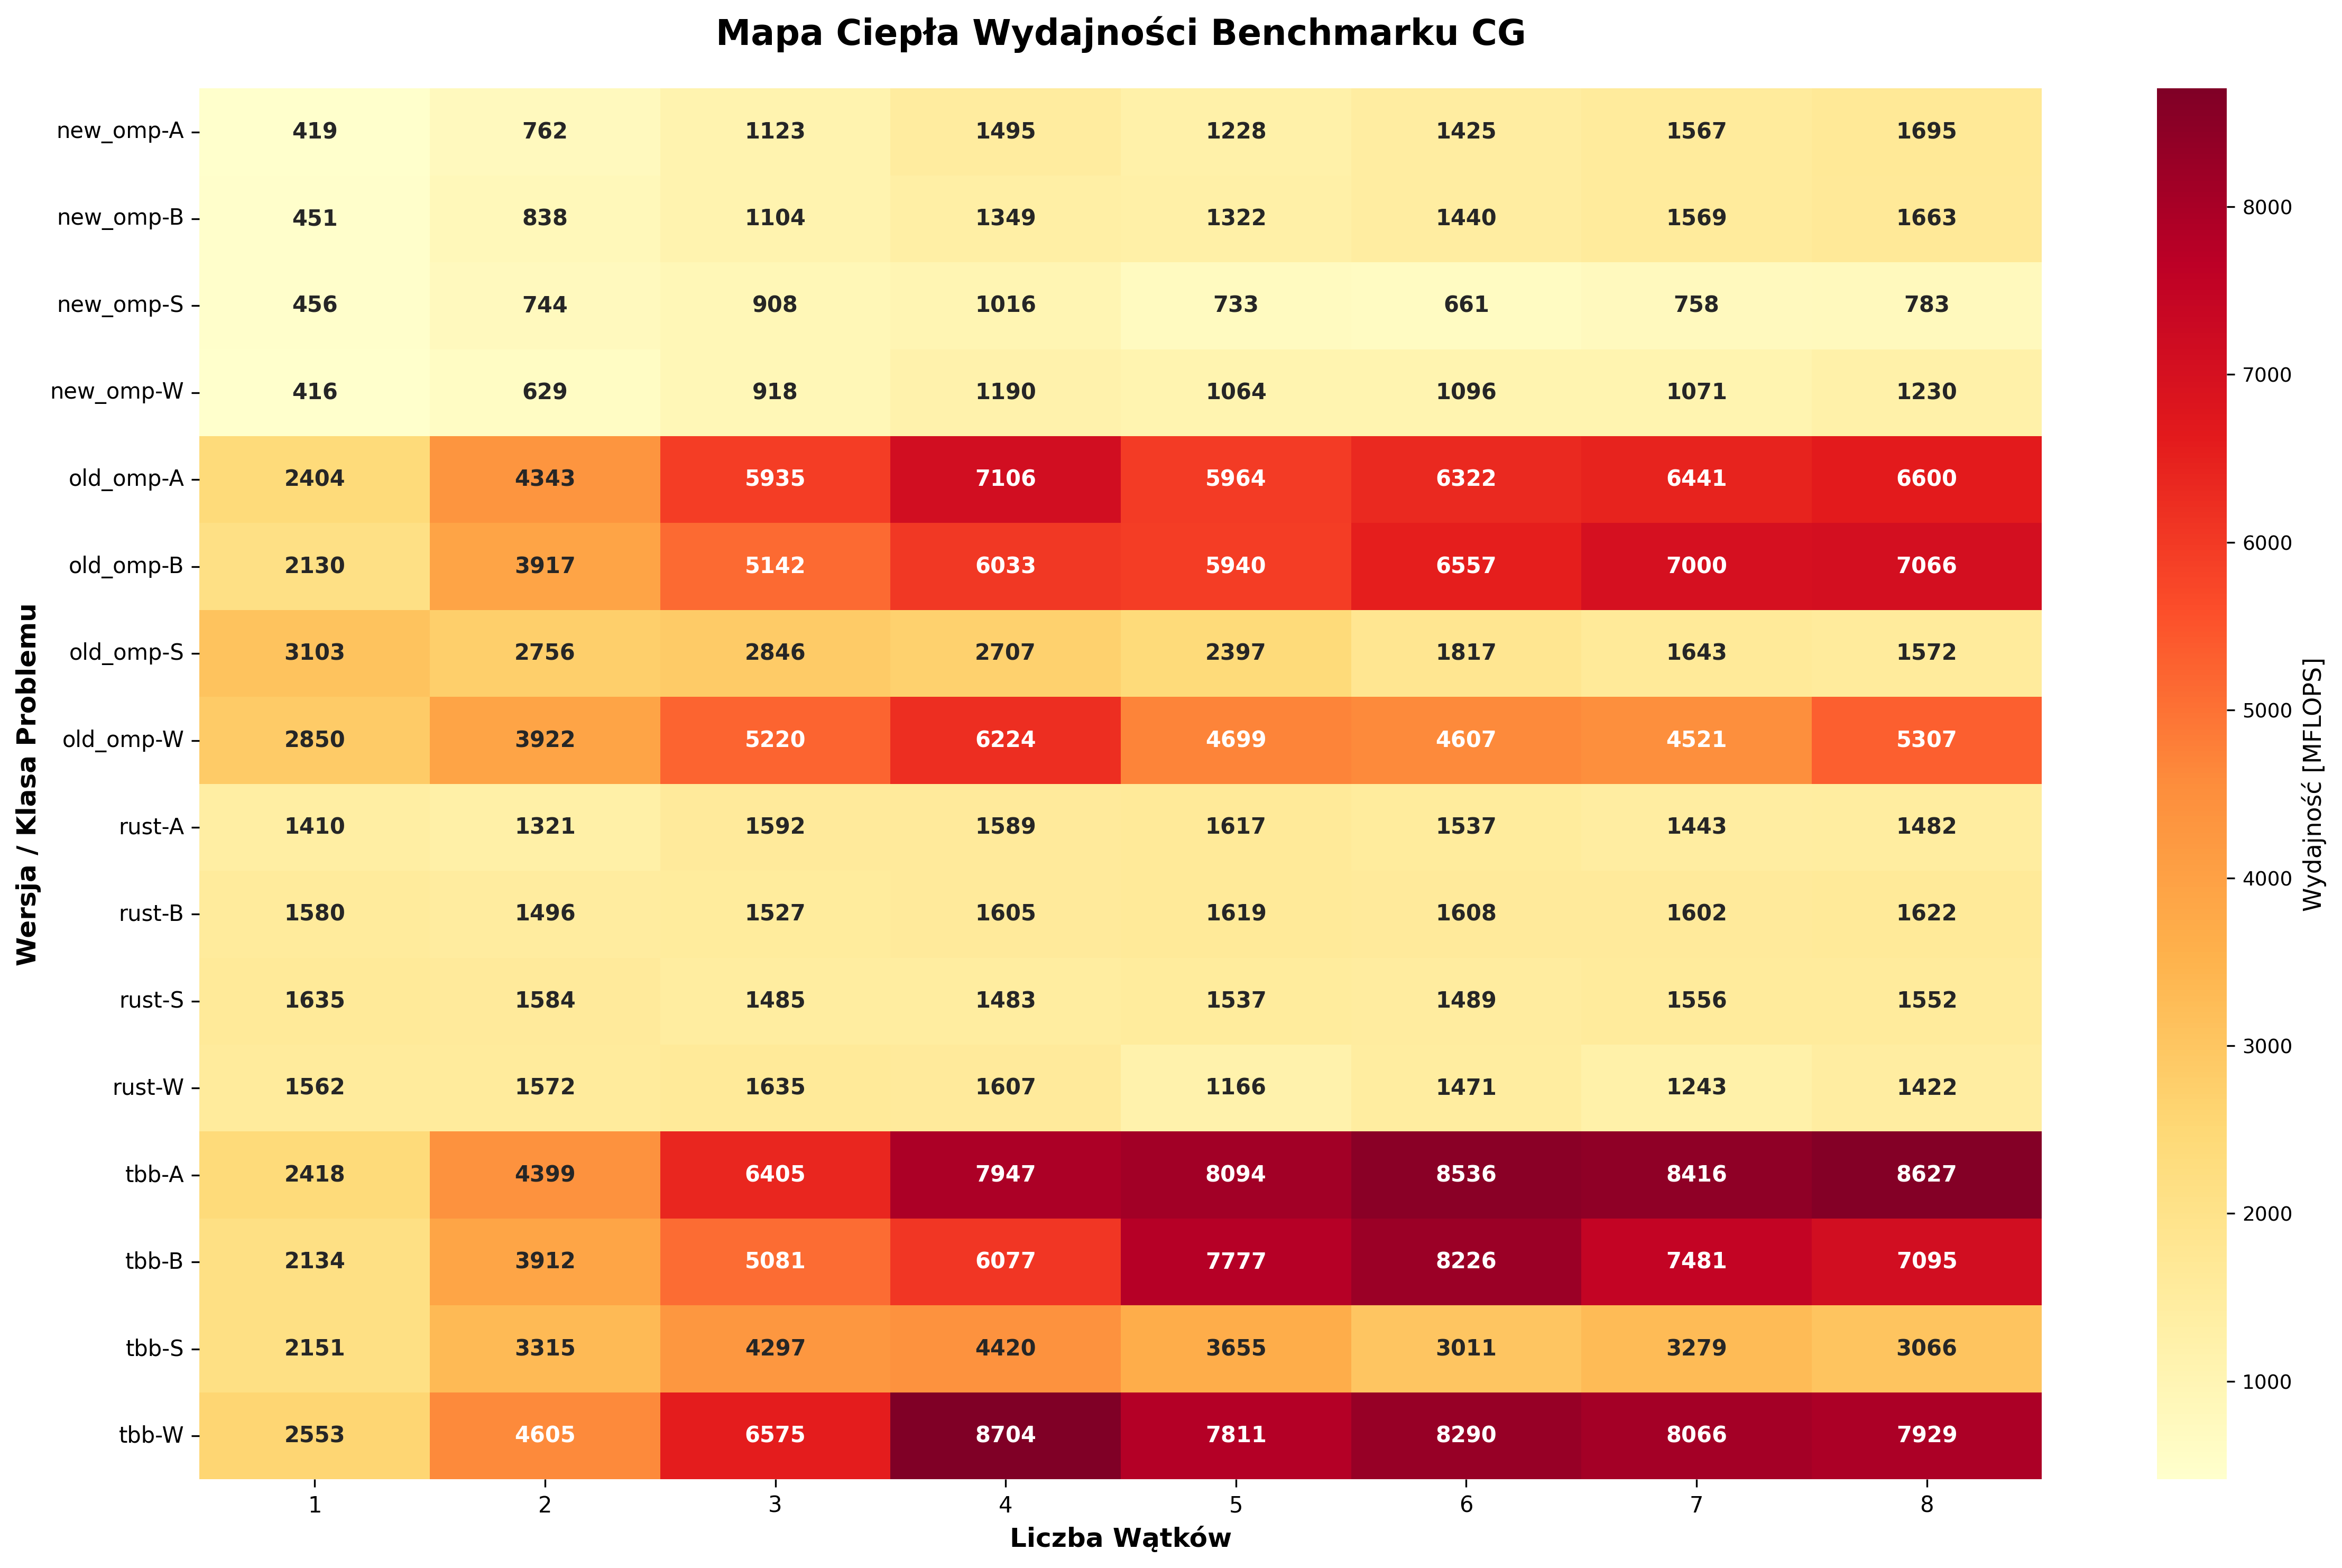
\includegraphics[width=\textwidth]{analiza/images/parallel/cg/cg_mapa_ciepla_wydajnosci.png}
    \caption{Mapa ciepła wydajności benchmarku CG dla klas S, W, A, B względem liczby użytych wątków}
    \label{cg_heatmap_wydajnosci}
\end{figure}
Powyższa mapa cieplna - rysunek \ref{cg_heatmap_wydajnosci} przedstawia wydajność (w MFLOPS). Wydajność została przedstawiona w zależności od liczby użytych wątków. Odcienie koloru od żółtego do ciemnoczerwonego wskazują na wzrost wydajności.

\begin{figure}[H]
    \centering
    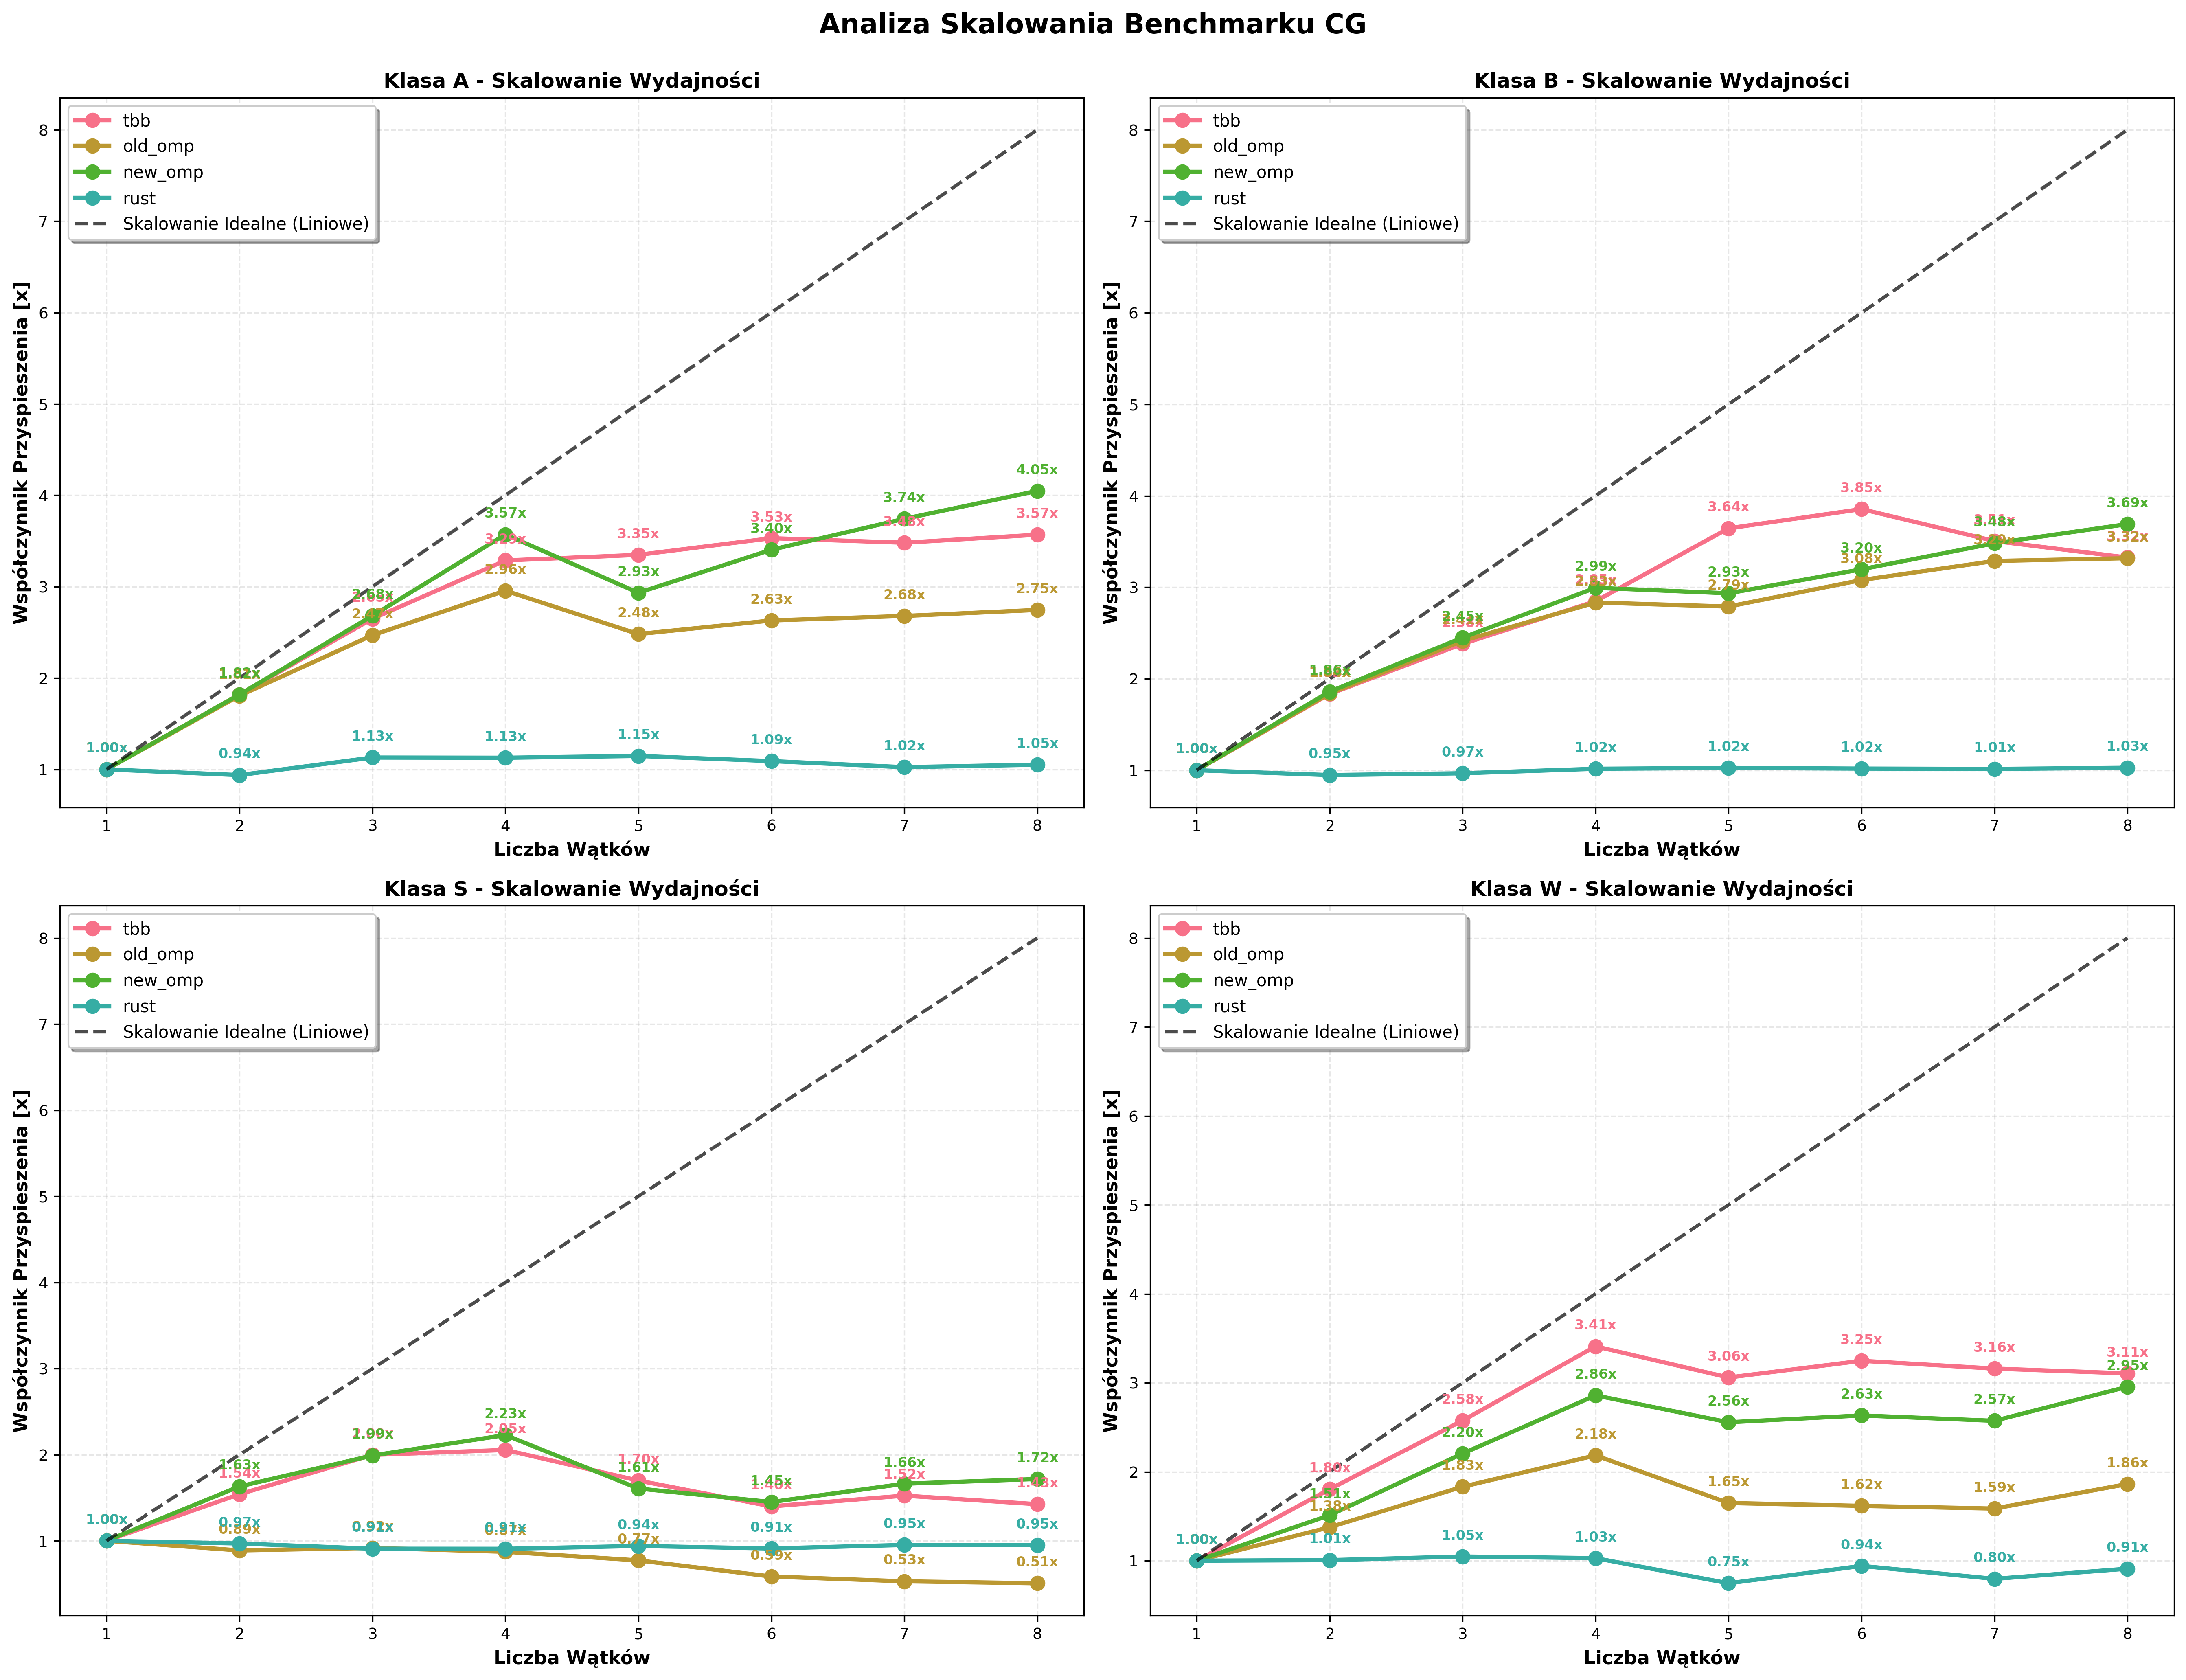
\includegraphics[width=\textwidth]{analiza/images/parallel/cg/cg_analiza_skalowania.png}
    \caption{Analiza skalowania benchmarku CG dla klas S, W, A, B względem liczby użytych wątków}
    \label{cg_analiza_skalowania}
\end{figure}
Powyższy wykres - rysunek \ref{cg_analiza_skalowania} przedstawia skalowanie wydajności benchmarku CG. Skalowanie wyrażone zostało za pomocą współczynnika przyspieszenia względem wykonania jednowątkowego i odniesione do skalowania idealnego (liniowego).

\subsubsection{Klasa S}
W klasie S, ze względu na niewielki rozmiar problemu, skalowanie jest ograniczone:
\begin{itemize}
    \item TBB osiąga maksimum przy 3 wątkach (~4297 MFLOPS), a następnie wydajność spada - jest to zgodne z typowym zjawiskiem nadmiaru wątków dla małych danych.
    \item old\_omp zachowuje się podobnie - osiąga maksimum przy 3 wątkach, a następnie stopniowo traci wydajność, spadając poniżej 2000 MFLOPS przy 6-8 wątkach.
    \item new\_omp rośnie stopniowo do ok. 900 MFLOPS, jednak bez dalszych wzrostów - potwierdzając małą efektywność tej wersji OpenMP w przypadku małych problemów.
    \item Rust utrzymuje bardzo stabilny poziom (~1500 MFLOPS), przewyższając new\_omp, lecz nie osiągając wartości TBB czy old\_omp.
    \item wszystkie implementacje wykazują ograniczone zdolności do skalowania. TBB i old\_omp osiągają maksymalne przyspieszenie rzędu ~1,7x, new\_omp i rust oscylują wokół 1x lub wręcz wykazują pogorszenie wydajności wraz ze wzrostem liczby wątków. Wskazuje to na narzut związany z zarządzaniem wątkami, który w przypadku małych problemów dominuje nad potencjalnym zyskiem z równoległości.
\end{itemize}

\subsubsection{Klasa W}
Na wykresie dla klasy W widać znaczną różnicę w wydajności między implementacjami:
\begin{itemize}
    \item TBB osiąga najwyższą wydajność, przekraczając 8000 MFLOPS przy 4 wątkach i stabilizując się w przedziale 8200-8500 MFLOPS dla 6-8 wątków.
    \item old\_omp osiąga dobre rezultaty, maksymalnie 5307 MFLOPS przy 8 wątkach, ale z niższą skalowalnością.
    \item new\_omp nie przekracza 1400 MFLOPS, a jego krzywa ma charakter niemal liniowy.
    \item Rust notuje wartości w zakresie 1500-1600 MFLOPS przy 1-4 wątkach, z tendencją spadkową przy większym obciążeniu, co może wskazywać na problemy z efektywną synchronizacją.
    \item TBB osiąga przyspieszenie rzędu 3,11x, old\_omp oraz rust nieznacznie poniżej tego poziomu (2,5-3x). new\_omp ponownie wypada słabo, kończąc na poziomie ~1,66x dla 8 wątków. Ograniczona skalowalność new\_omp może wynikać z nieefektywnego zarządzania regionami równoległymi lub braku adaptacji do większych problemów obliczeniowych.
\end{itemize}


\subsubsection{Klasa A}
W klasie A obserwujemy znacznie lepsze wyniki wydajności:
\begin{itemize}
    \item TBB osiąga najwyższą wydajność spośród wszystkich implementacji, dochodząc do wartości około 8627 MFLOPS przy 8 wątkach. Krzywa TBB rośnie monotonnie aż do 6 wątków, po czym stabilizuje się.
    \item old\_omp osiąga szczytową wydajność przy 3 wątkach (7350 MFLOPS), następnie wydajność delikatnie spada i stabilizuje się w zakresie 6100-6300 MFLOPS.
    \item new\_omp wykazuje niską wydajność - rosnącą do poziomu ~1700 MFLOPS przy 8 wątkach - wskazując na mniejszą efektywność względem pozostałych implementacji C/C++.
    \item Rust utrzymuje się na poziomie ~1400 MFLOPS i nie wykazuje znaczącej poprawy przy wzroście liczby wątków.
    \item najbardziej efektywne skalowanie osiąga implementacja TBB, z przyspieszeniem dochodzącym do około 4,05x przy 8 wątkach. old\_omp oraz rust osiągają zbliżone przyspieszenia (ok. 3,5x), natomiast new\_omp cechuje się słabym skalowaniem, zatrzymując się poniżej 1,2x. Oznacza to, że nowa implementacja OpenMP (new\_omp) nie potrafi w pełni wykorzystać dostępnych zasobów w tej klasie problemu.
\end{itemize}

\subsubsection{Klasa B}
W klasie B, ze względu na większą złożoność problemu, wydajność jest znacznie niższa:
\begin{itemize}
    \item Również w tej klasie TBB dominuje pod względem wydajności - osiągając maksimum 8266 MFLOPS przy 6 wątkach, chociaż dla 8 wątków obserwujemy spadek (7143 MFLOPS), co może sugerować efekt przeciążenia zasobów.
    \item old\_omp wykazuje niemal liniowy wzrost wydajności, kończąc na poziomie 7090 MFLOPS, co czyni tę implementację bardzo stabilną i skalowalną.
    \item new\_omp poprawia wydajność wraz ze wzrostem liczby wątków, lecz kończy na poziomie 1662 MFLOPS - podobnie jak w klasie A, co potwierdza jej relatywnie niską efektywność.
    \item Rust utrzymuje stałą wydajność na poziomie ~1580-1600 MFLOPS, wykazując bardzo małą czułość na liczbę wątków.
    \item zaobserwować można zbliżone zależności jak w klasie A. TBB dominuje skalowaniem (do 3,85x), choć z mniejszym przyrostem niż w klasie A. old\_omp, rust i new\_omp pozostają w zakresie przyspieszeń rzędu 3,0-3,7x. new\_omp nadal wykazuje istotnie słabsze skalowanie w porównaniu do pozostałych bibliotek, a jego przyrosty wydajności od 4 do 8 wątków są marginalne.
\end{itemize}

Analiza mapy cieplnej \ref{cg_heatmap_wydajnosci} jednoznacznie wskazuje, że najlepszą ogólną wydajność oraz skalowalność wykazują implementacje wykorzystujące bibliotekę TBB, zwłaszcza dla dużych klas problemu (A, B, W). Starsze implementacje OpenMP również oferują konkurencyjną wydajność, jednak ich efektywność jest mniej stabilna przy rosnącej liczbie wątków. W porównaniu do tych rozwiązań, nowe wersje OpenMP oraz implementacje w języku Rust pozostają wyraźnie mniej wydajne i słabiej skalowalne, co może wskazywać na potrzebę dalszych optymalizacji lub ograniczenia środowiska uruchomieniowego.


\subsection{Wnioski z benchmarku CG}
Z analizy wykresu \ref{cg_porownanie_czasow_wykonania} można wyciągnąć następujące wnioski:

Skalowalność implementacji różni się w zależności od klasy problemu i użytej technologii. Implementacje TBB oraz OpenMP (szczególnie starsza wersja) wykazują dobrą skalowalność w większości przypadków.

Rust oferuje wyjątkowo dobre czasy wykonania dla dużych problemów (klasa A i B), lecz jego stabilność wydajności dla klasy W i S budzi wątpliwości, szczególnie przy małej liczbie danych.

OpenMP (new\_omp) wykazuje potencjał skalowania, lecz jego czasy wykonania są często wyższe niż w przypadku TBB lub old\_omp, co może wynikać z narzutu nowszych konstrukcji.

W klasach problemu o małej skali (S, częściowo W) zwiększanie liczby wątków nie zawsze przynosi poprawę wydajności, a czasem wręcz ją pogarsza - co jest zgodne z klasycznymi obserwacjami dotyczącymi wpływu narzutu synchronizacji przy małych danych.

Analizując wykres rysunku \ref{cg_porownanie_wydajnosci}, można zauważyć, że:

TBB jest najwydajniejszą implementacją dla większości klas problemów (A, B, W), z wyjątkiem klasy S, gdzie obserwuje się spadek efektywności przy większej liczbie wątków.

Old\_omp wykazuje dobrą skalowalność, choć jej wydajność jest nieco niższa niż TBB - szczególnie w większych klasach (A, B).

New\_omp osiąga najniższe wyniki we wszystkich klasach, co może wynikać z zastosowania bardziej złożonych mechanizmów synchronizacji.

Rust, mimo bardzo stabilnych wyników, nie osiąga konkurencyjnych poziomów wydajności - zwłaszcza przy większych problemach - jednak jego zachowanie może być zaletą w kontekście deterministycznych systemów lub środowisk o ograniczonych zasobach.


\subsection{Wyniki benchmarków - platforma x86\_64}
%------------------------------
%------------------------------
\subsection{Wyniki profilowania wydajności - platforma ARM64}
\begin{figure}[H]
    \centering
    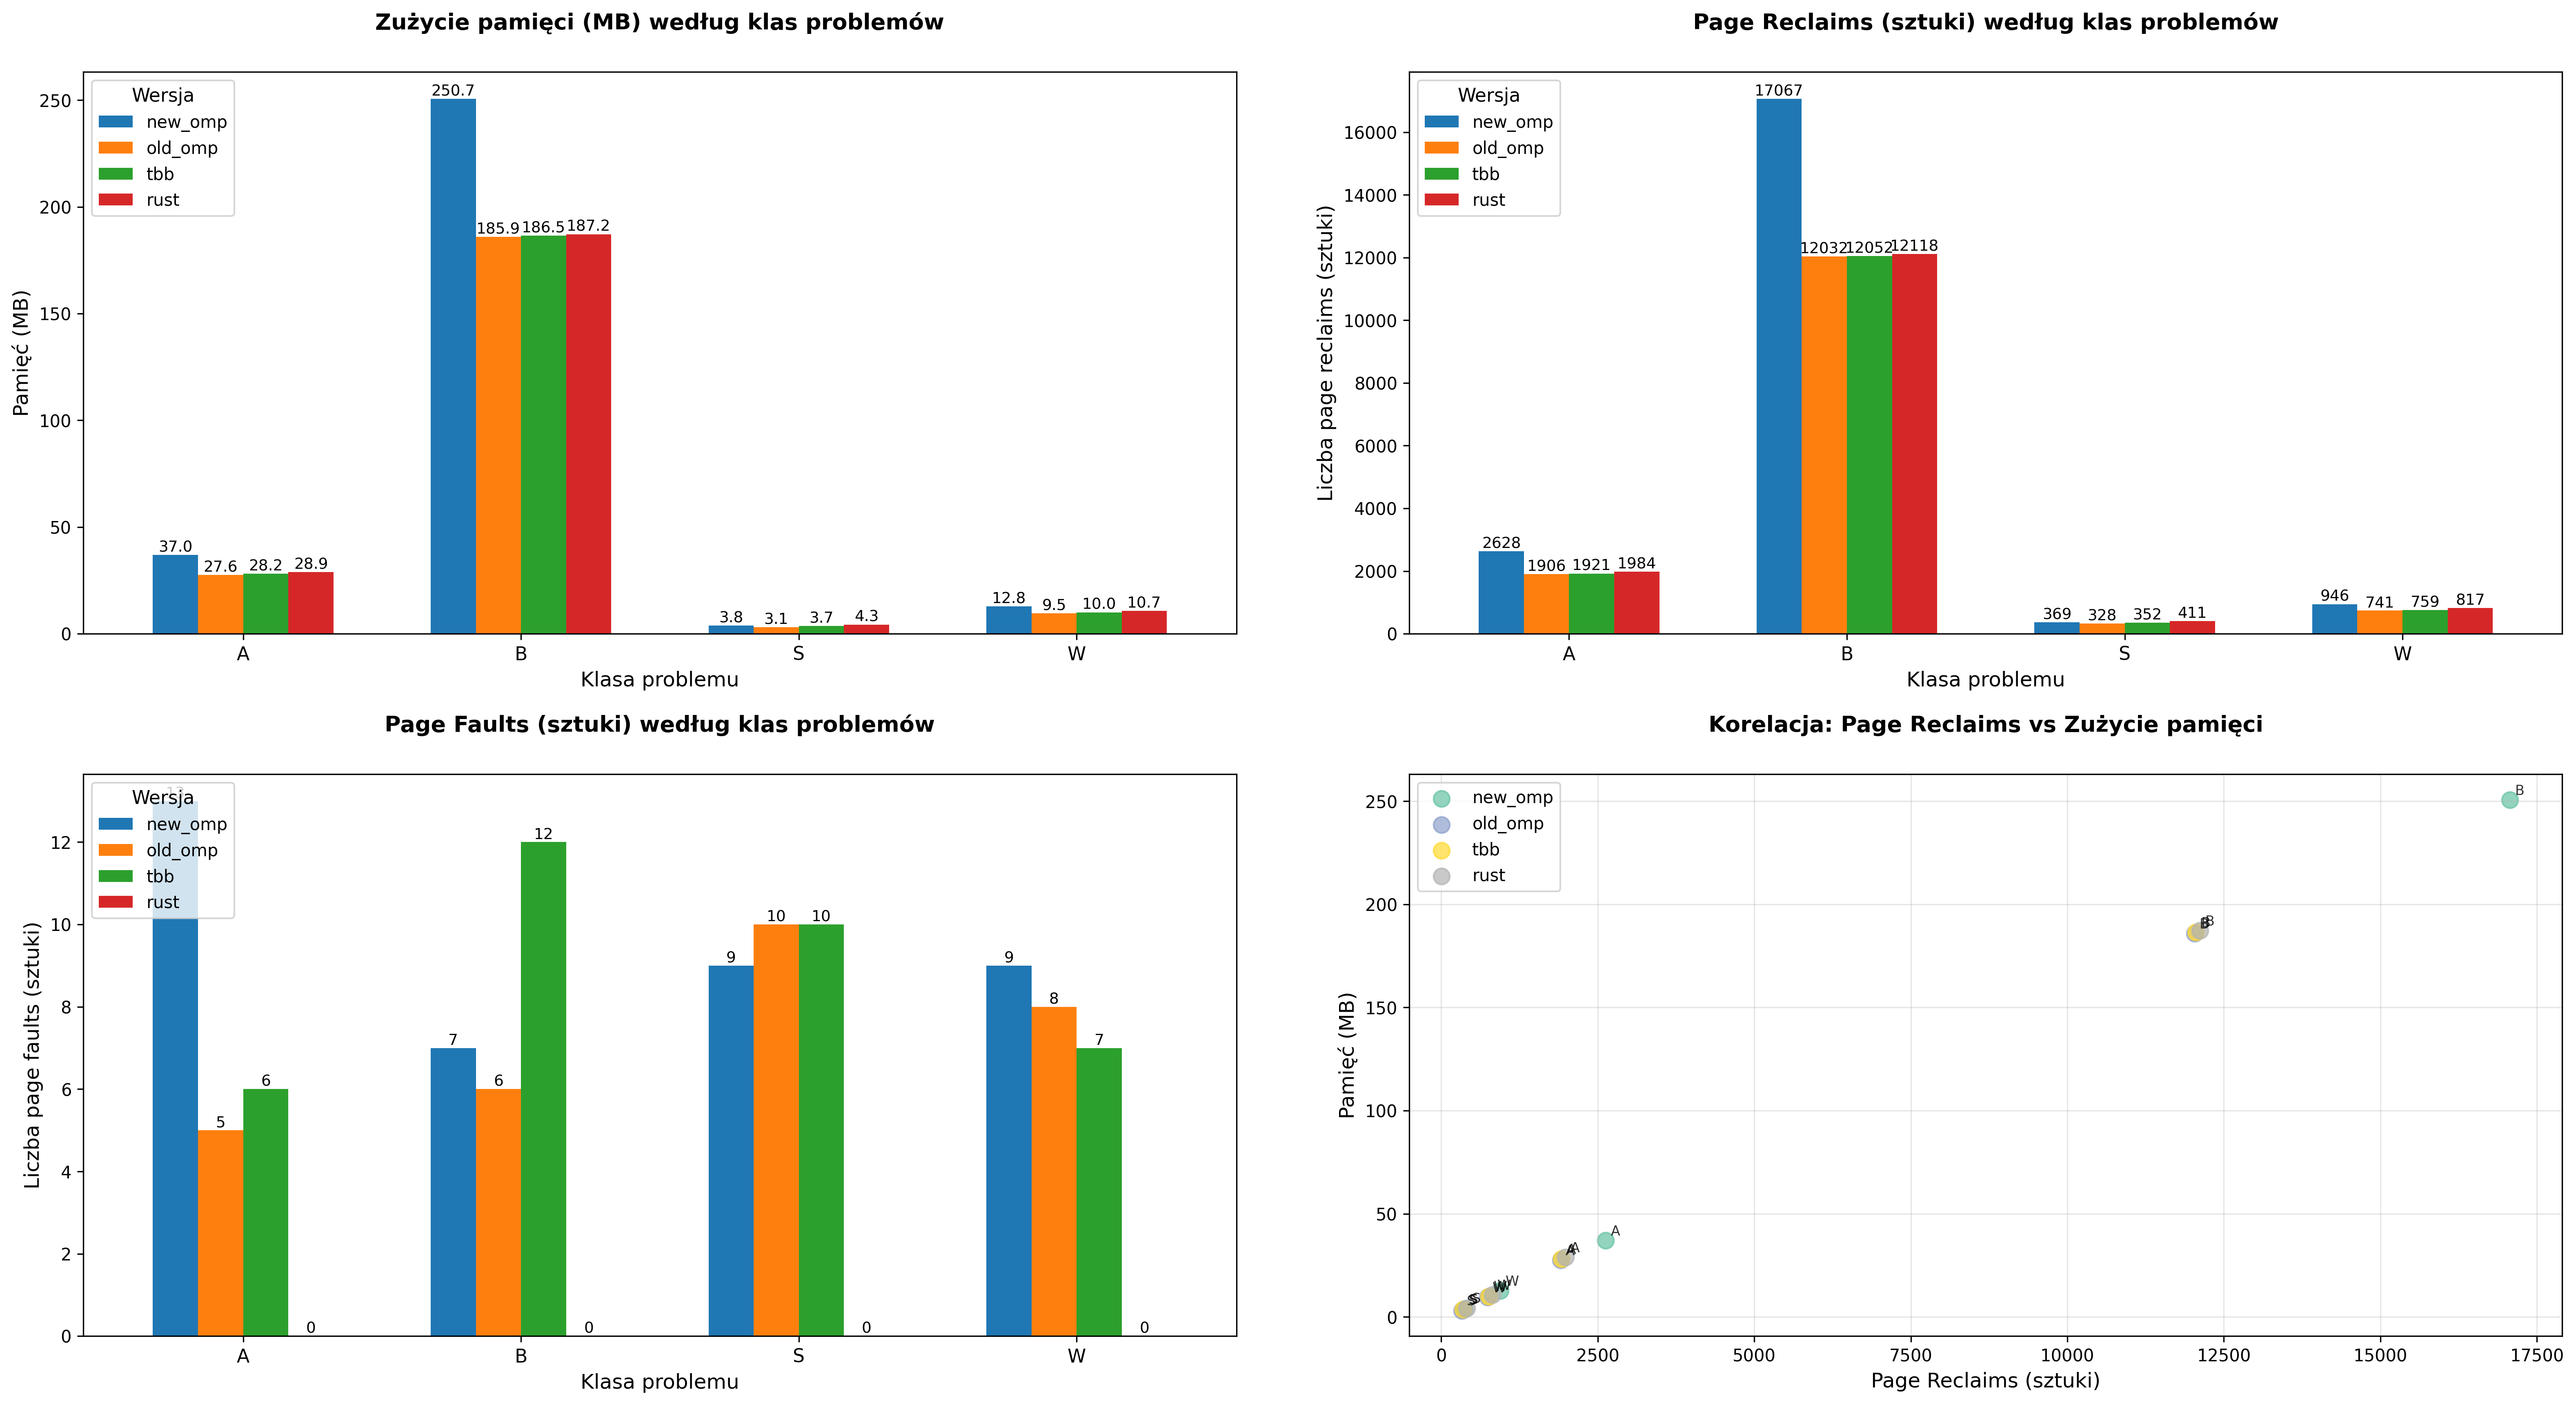
\includegraphics[width=\textwidth]{analiza/images/parallel/cg/chart_01_memory_comparison.png}
    \caption{Profilowanie wydajności benchmarku CG dla klas S, W, A, B względem liczby użytych wątków}
    \label{cg_porownanie_zuzycia_pamieci}
\end{figure}

\subsubsection{Zużycie pamięci (MB)}
Na pierwszym wykresie - rysunek \ref{cg_porownanie_zuzycia_pamieci} (lewy górny róg) przedstawiono zużycie pamięci operacyjnej (w MB) dla czterech wersji implementacji algorytmu:
\begin{itemize}
    \item W klasie problemu B występuje najwyższe zużycie pamięci we wszystkich wersjach. Szczególnie zauważalny jest wynik dla new\_omp (250,7 MB), który znacząco przekracza wartości dla pozostałych wersji (około 185-187 MB).
    \item W klasie A new\_omp również zużywa najwięcej pamięci (37 MB), natomiast pozostałe wersje wykazują zbliżony i niższy poziom zużycia (około 27-29 MB).
    \item W klasach S i W różnice są mniej wyraźne, jednak nadal new\_omp wykazuje największe zużycie pamięci.
    \item Wersja rust generalnie charakteryzuje się najmniejszym lub jednym z najmniejszych zużyć pamięci w większości klas problemów.
\end{itemize}

\subsubsection{Liczba zwalniania stron pamięci (sztuki)}
Drugi wykres - rysunek \ref{cg_porownanie_zuzycia_pamieci} (prawy górny róg) ilustruje liczbęzwalniania stron pamięci \eng{page reclaim}, czyli sytuacji, w których system operacyjny odzyskuje strony pamięci.
\begin{itemize}
    \item Najwięcej zwalnianych stron pamięci występuje w klasie B dla wersji new\_omp (17067), co koresponduje z jej wysokim zużyciem pamięci.
    \item W pozostałych wersjach liczba zwolnionych stron w klasie B jest znacznie niższa (około 12000-12100).
    \item W klasie A new\_omp ponownie osiąga najwyższy wynik (2628), przy niższych wartościach pozostałych wersji (około 1900).
    \item W klasach S i W różnice są mniej zauważalne, choć new\_omp nadal wykazuje wyższe wartości.
\end{itemize}

\subsubsection{Odwołania do nieobecnych stron (sztuki)}
Trzeci wykres - rysunek \ref{cg_porownanie_zuzycia_pamieci} (lewy dolny róg) przedstawia odwołania do nieobecnych stronliczbę \eng{page fault} - czyli sytuacji, w których wymagany fragment pamięci nie znajduje się aktualnie w RAM-ie.
\begin{itemize}
    \item W klasie A new\_omp wykazuje najwyższą liczbę page faults (13), zaś rust nie generuje żadnych błędów.
    \item W klasie B najwięcej błędów generuje TBB (12), podczas gdy rust ponownie nie wykazuje żadnych.
    \item W klasach S i W rust również nie generuje page faults, a inne wersje wykazują umiarkowane wartości (7-10).
    \item Wyniki te sugerują bardzo efektywną gospodarkę pamięciową w wersji rust.
\end{itemize}

\subsubsection{Korelacja: Liczba zwalniania stron pamięci vs Zużycie pamięci}
Ostatni wykres - rysunek \ref{cg_porownanie_zuzycia_pamieci} (prawy dolny róg) ilustruje zależność pomiędzy liczbą zwolnionych stron pamięci a zużyciem pamięci.
\begin{itemize}
    \item Widoczna jest silna dodatnia korelacja - im większe zużycie pamięci, tym większa liczba zwolnionych stron pamięci. Najwyraźniejszym punktem odniesienia jest wersja new\_omp dla klasy B, która dominuje pod względem obu metryk.
    \item Punkty reprezentujące wersję rust znajdują się w lewej dolnej części wykresu, wskazując na niskie zużycie pamięci i małą liczbę zwolnionych stron.
\end{itemize}

\begin{figure}[H]
    \centering
    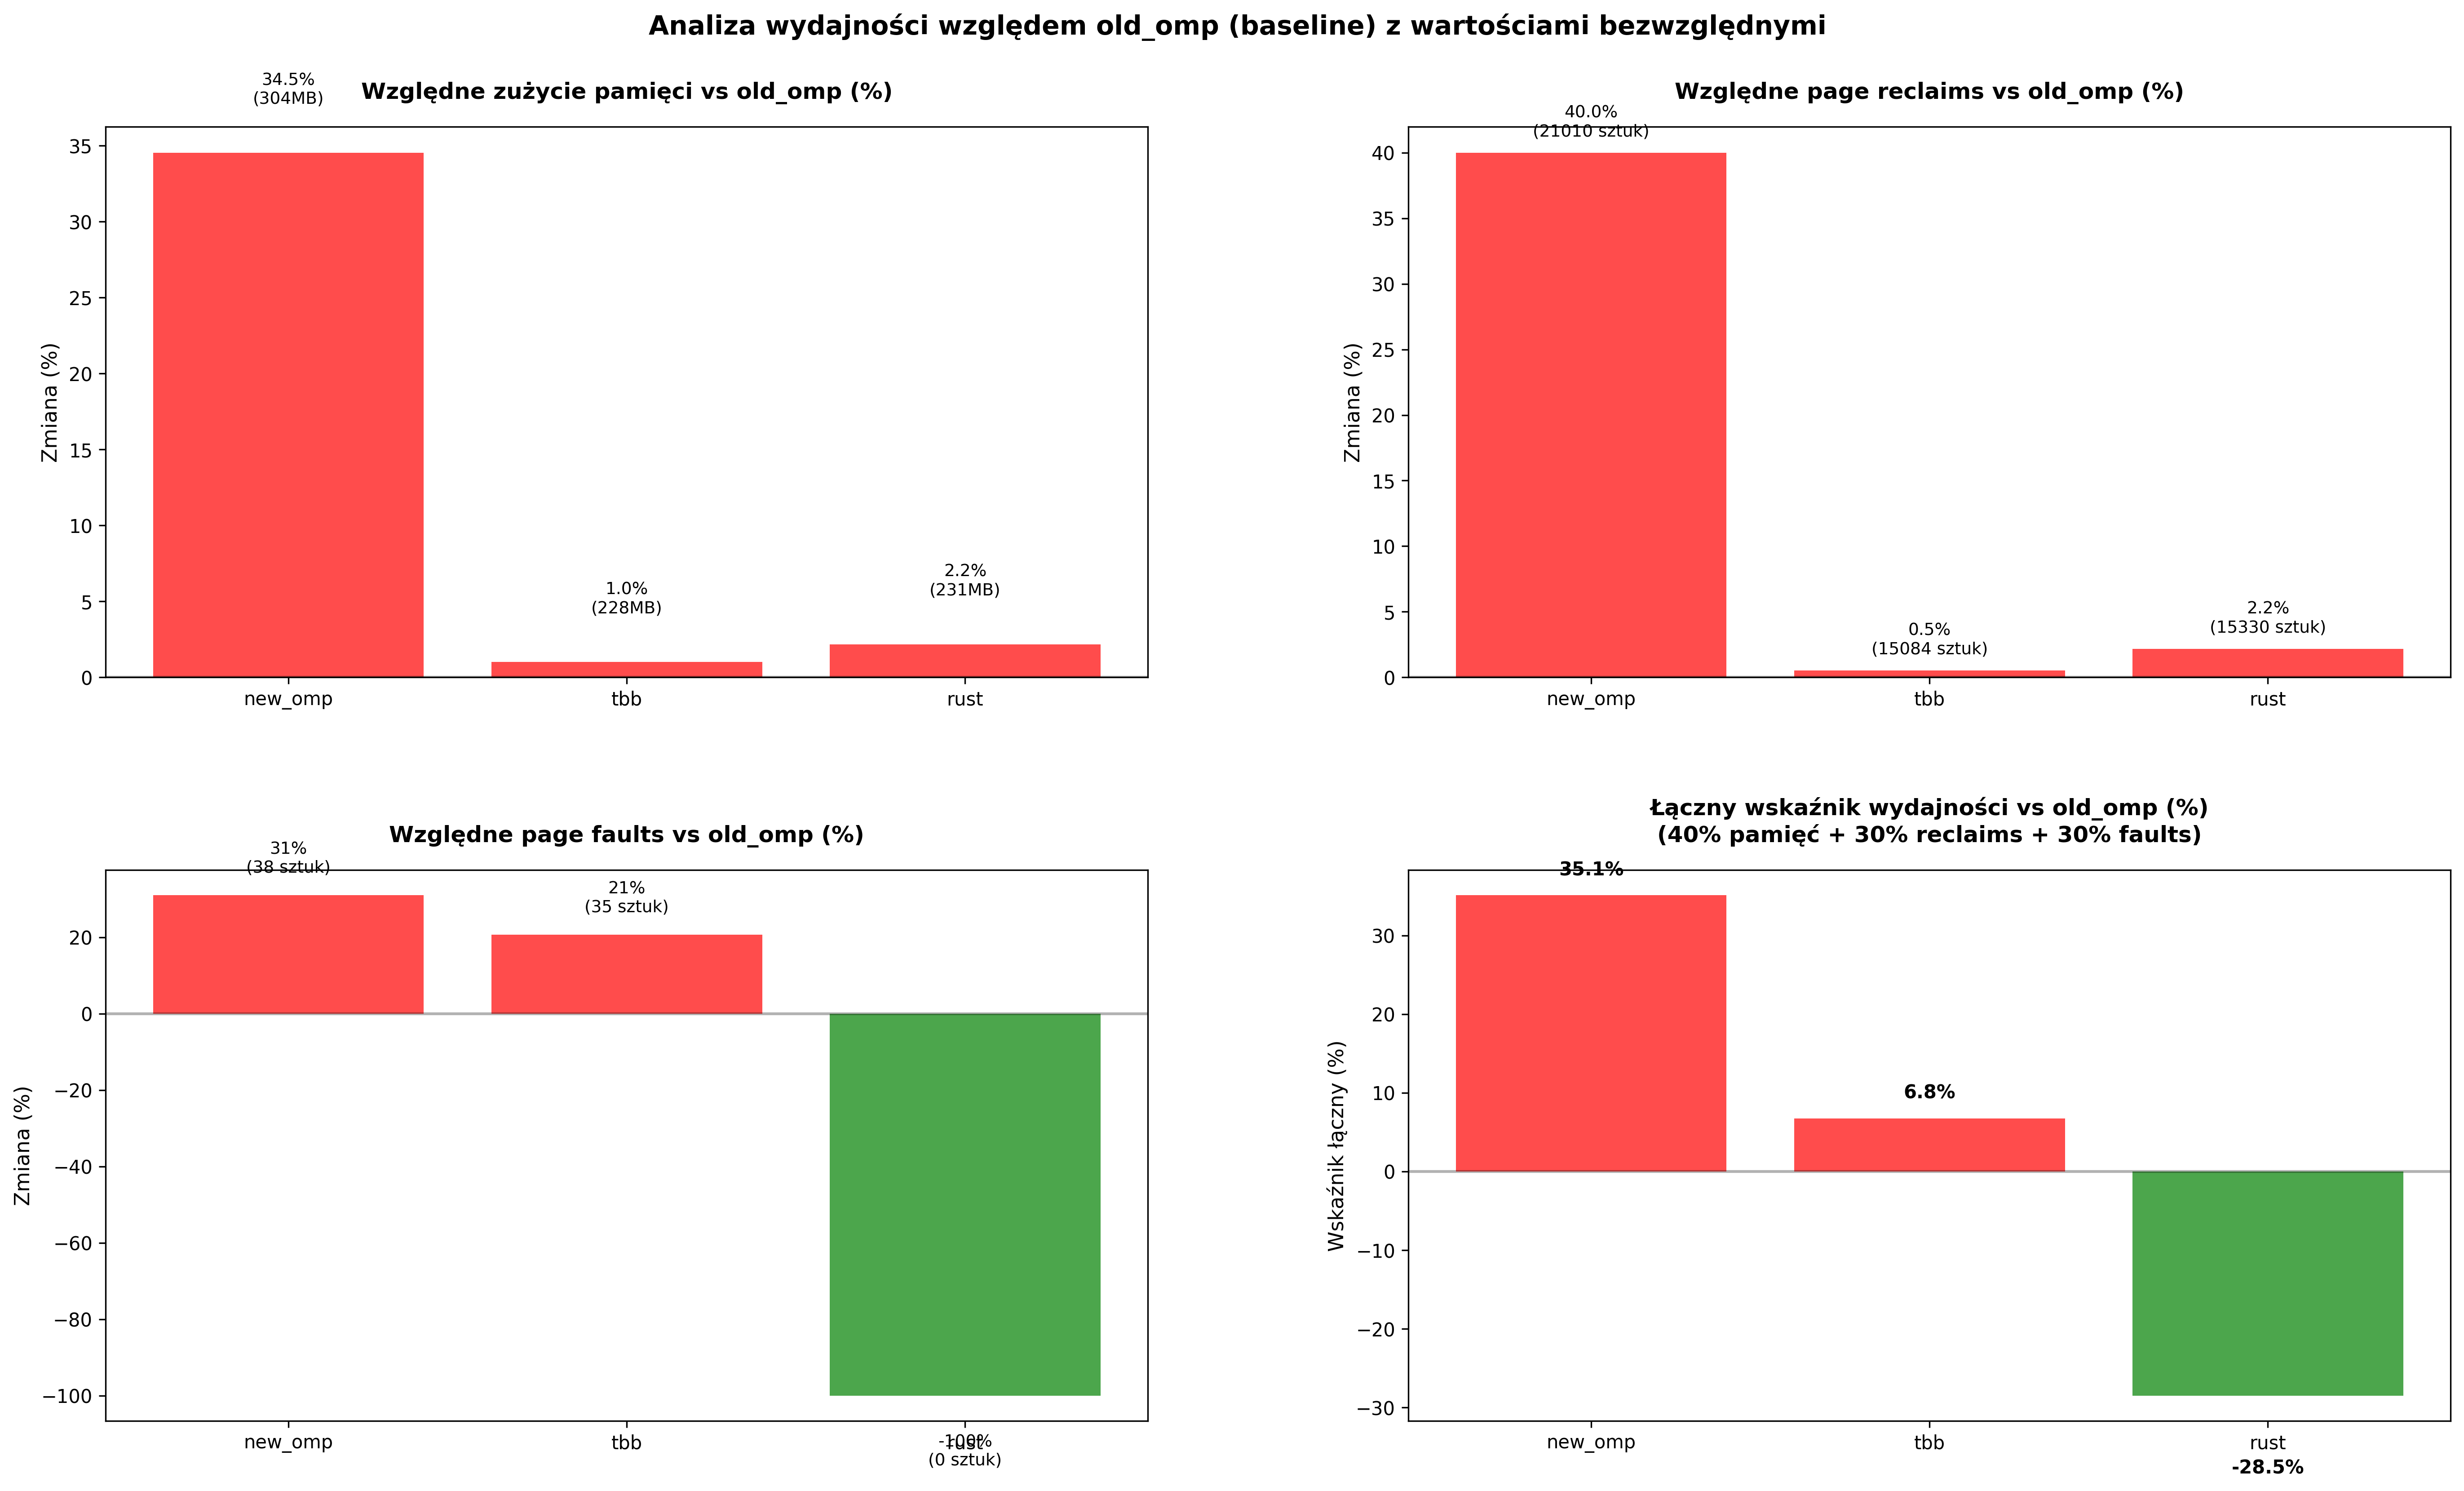
\includegraphics[width=\textwidth]{analiza/images/parallel/cg/chart_05_performance_ratios.png}
    \caption{Analiza wydajności względem old\_omp (punkt odniesienia) z wartościami bezwzględnymi}
    \label{cg_analiza_wzgledem_old_omp}
\end{figure}
Na wykresie - rysunek \ref{cg_analiza_wzgledem_old_omp} szczegółowa analiza czterech wykresów przedstawiających względną wydajność trzech wersji implementacji (new\_omp, TBB, rust) względem wersji bazowej old\_omp. Analiza dotyczy zużycia pamięci, liczby zwolnionych stron pamięci, odwołań do nieobecncyh stron oraz skumulowanego wskaźnika efektywności.
\subsubsection{Względne zużycie pamięci vs old\_omp}
Pierwszy wykres - rysunek \ref{cg_analiza_wzgledem_old_omp} (lewy górny róg) ukazuje procentową zmianę w zużyciu pamięci operacyjnej względem implementacji referencyjnej. Największy wzrost odnotowano dla new\_omp, gdzie zużycie pamięci wzrosło o 34,5\%, co przekłada się na dodatkowe 304 MB. Zmiany dla TBB i rust były marginalne i wyniosły odpowiednio 1,0\% (228 MB) oraz 2,2\% (231 MB), co sugeruje ich większą efektywność w kontekście gospodarowania pamięcią.

\subsubsection{Względne odzyskiwanie stron pamięci vs old\_omp}
Drugi wykres - rysunek \ref{cg_analiza_wzgledem_old_omp} (prawy górny róg) przedstawia zmiany w liczbie odzyskanych stron pamięci. Implementacja new\_omp wykazała aż 40\% wzrost (21010 stron), co może świadczyć o intensywnym zarządzaniu pamięcią w trakcie wykonywania programu. Dla TBB i rust zmiany były minimalne (odpowiednio 0,5\% i 2,2\%), co może być interpretowane jako korzystny efekt optymalizacji dostępu do pamięci.

\subsubsection{Względne błędy stron vs old\_omp}
Na trzecim wykresie - rysunek \ref{cg_analiza_wzgledem_old_omp} (lewy dolny róg) obserwujemy względną liczbę błędów stron. new\_omp i TBB odnotowały wzrost liczby błędów stron odpowiednio o 31\% (38 sztuk) i 2\% (35 sztuk), co może wskazywać na mniej wydajne wykorzystanie pamięci w porównaniu z old\_omp. Z kolei rust jako jedyna implementacja odnotowała całkowitą eliminację błędów stron (-100\%, 0 sztuk), co potwierdza wyjątkowo skuteczną kontrolę pamięci operacyjnej - mechanizmy własności oraz pożyczania.

\subsubsection{Łączny wskaźnik wydajności vs old\_omp}
Na ostatnim wykresie - rysunek \ref{cg_analiza_wzgledem_old_omp} (prawy dolny róg) przedstawiono zagregowany wskaźnik wydajności, będący ważoną sumą trzech poprzednich metryk: 40\% udziału zużycia pamięci, 30\% udziału odzyskiwania stron oraz 30\% udziału błędów stron. Najwyższy wskaźnik (35,1\%) ponownie osiąga new\_omp, co oznacza wyraźnie wyższą konsumpcję zasobów w porównaniu do referencji. TBB wykazuje niewielki wzrost (6,8\%), co czyni go względnie neutralnym względem old\_omp. rust natomiast charakteryzuje się łącznym wskaźnikiem na poziomie -28,5\%, co czyni go najbardziej efektywną implementacją w ujęciu ogólnym.

\begin{figure}[H]
    \centering
    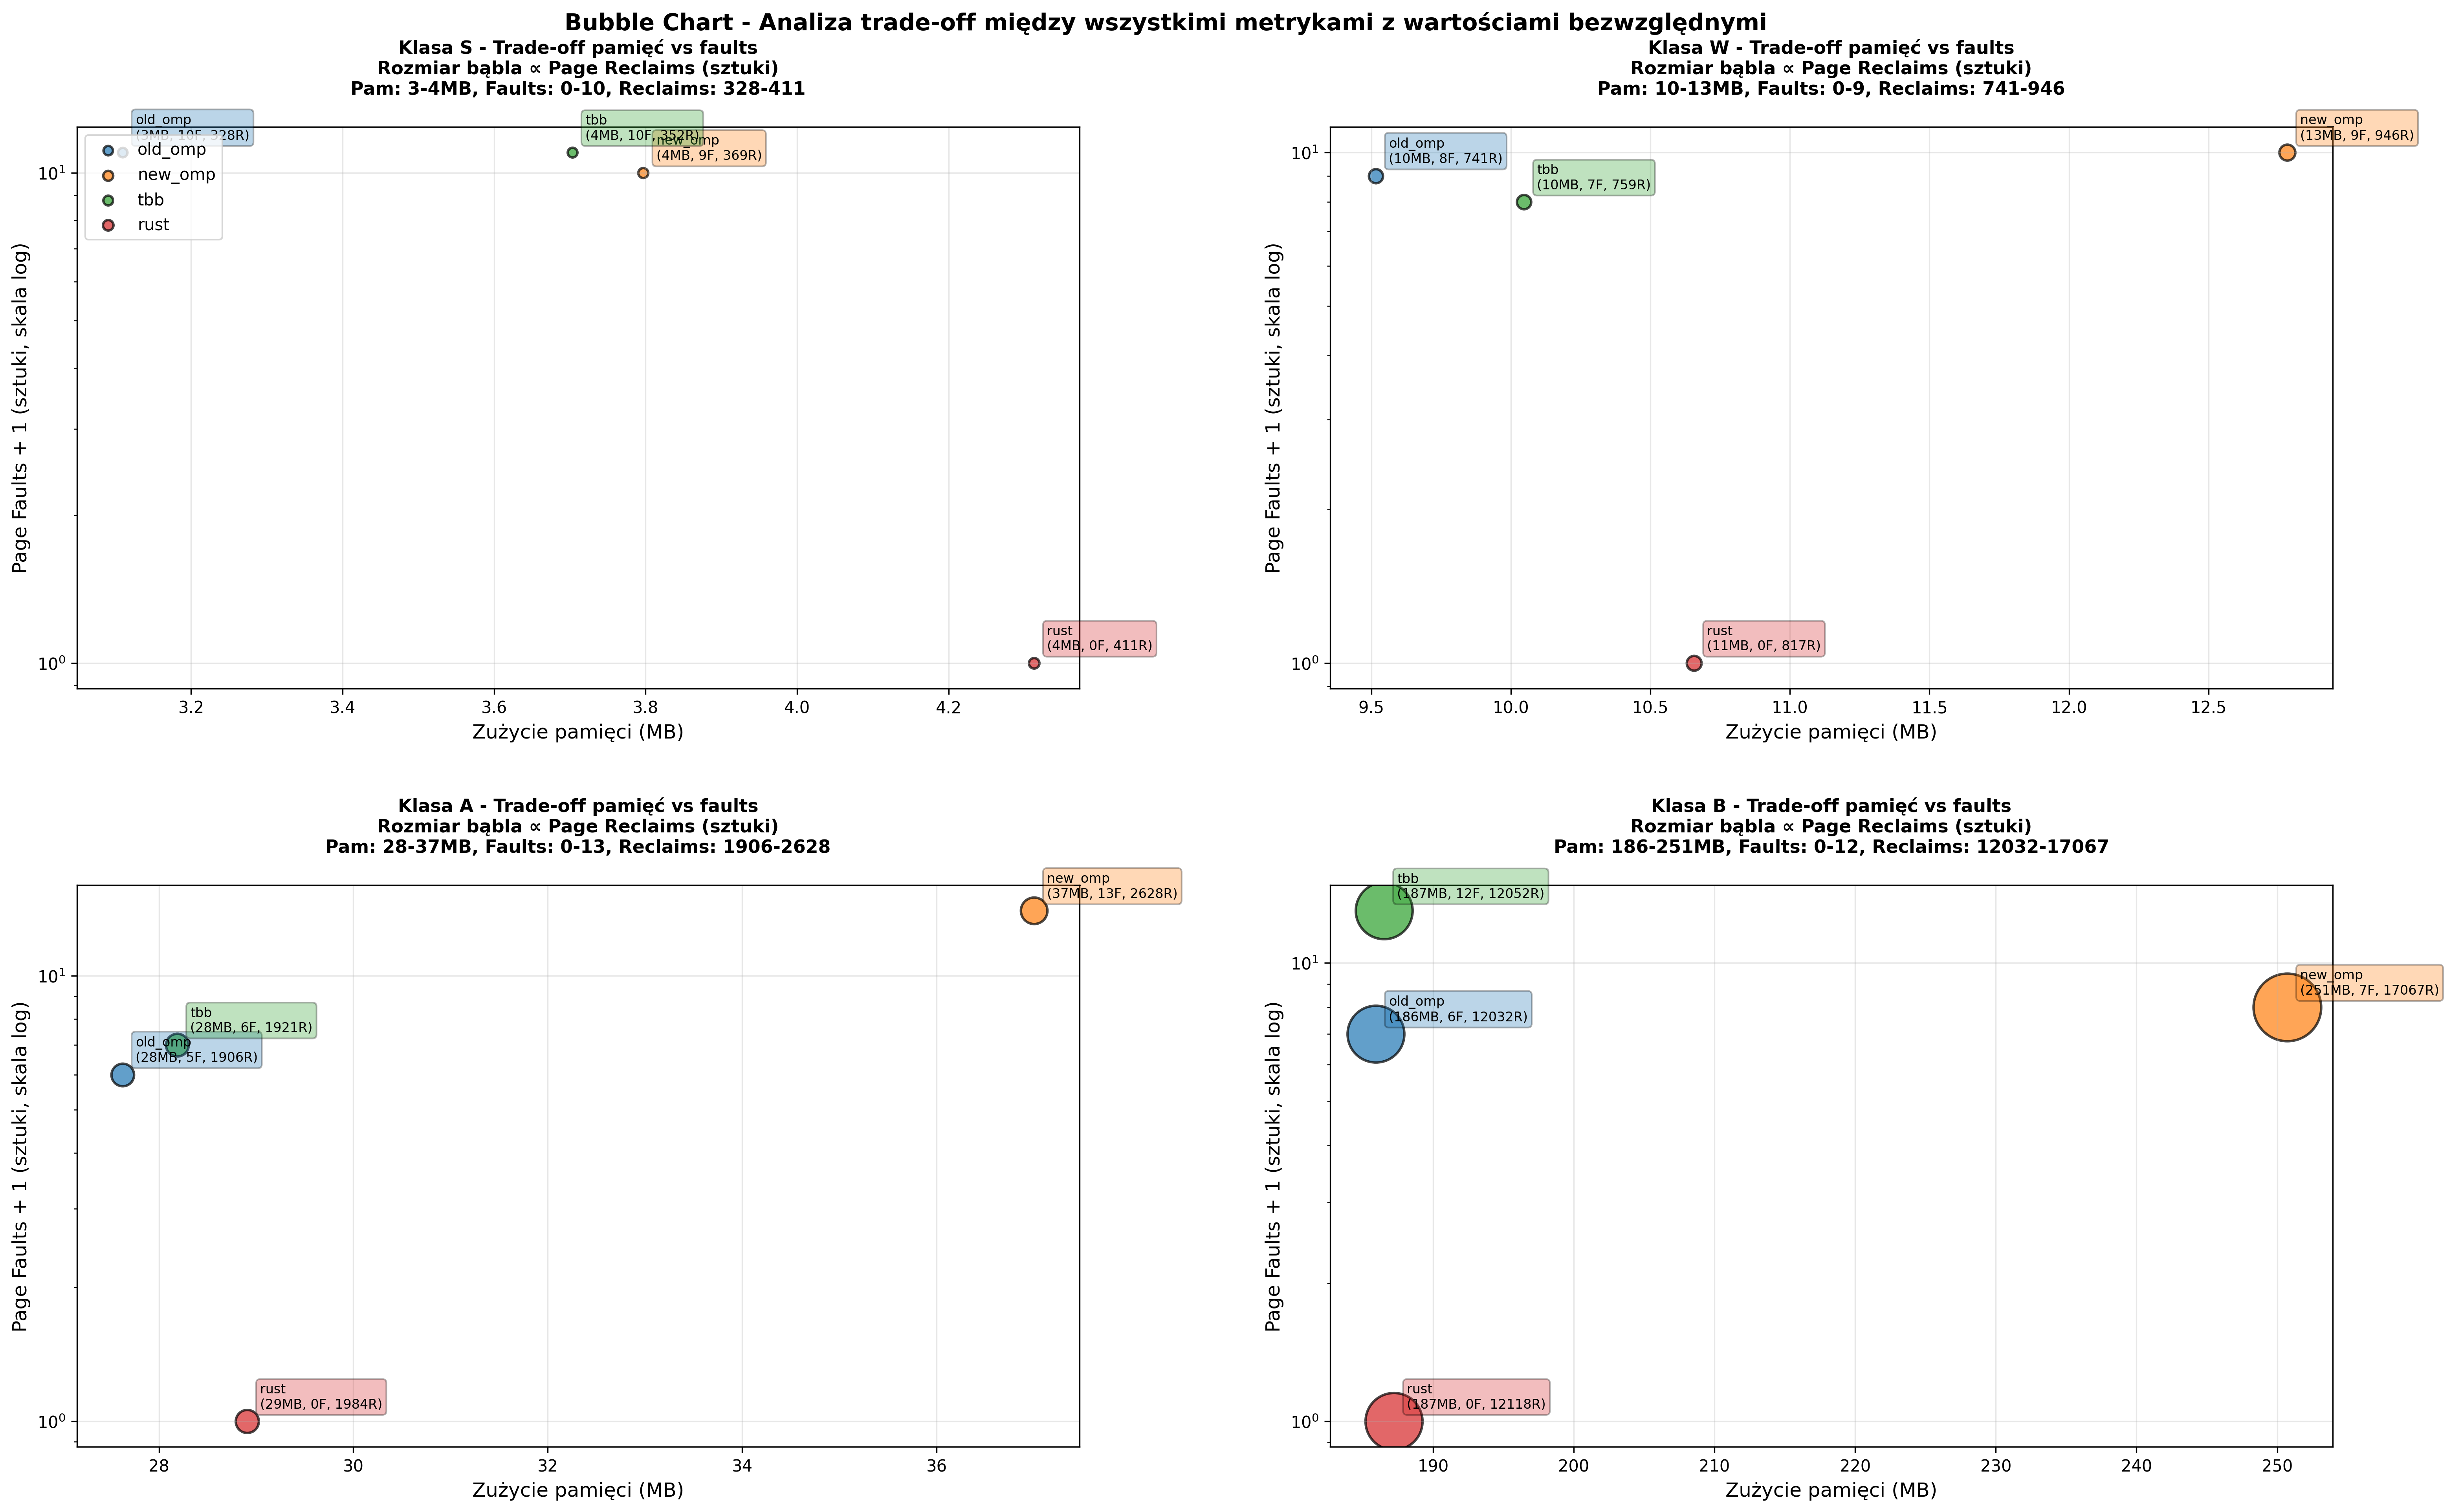
\includegraphics[width=\textwidth]{analiza/images/parallel/cg/chart_06_bubble_chart.png}
    \caption{Kompromisy \eng{trade-off} pomiędzy zużyciem pamięci a błędami stron pamięci, z uwzględnieniem liczby odzyskanych stron jako trzeciej zmiennej reprezentowanej przez rozmiar bąbla}
    \label{cg_kompromisy_pamiec_bledy}
\end{figure}

W celu całościowej oceny efektywności pamięciowej badanych implementacji, opracowano wykresy - rysunek \ref{cg_kompromisy_pamiec_bledy} typu "bubble chart”, które ukazują kompromisy między dwiema kluczowymi metrykami: zużyciem pamięci oraz liczbą błędów stron. Wykresy te wzbogacono o trzeci wymiar - liczbę odzyskanych stron pamięci, która została zakodowana poprzez rozmiar bąbla. Wszystkie wartości przedstawiono w postaci bezwzględnej, przy czym oś Y jest skalowana logarytmicznie w celu lepszego rozróżnienia niewielkich wartości.

Każdy z czterech wykresów odpowiada innej klasie obciążenia pamięciowego (S, W, A, B), przy czym wspólnym celem ich analizy jest uchwycenie relacji pomiędzy wzrostem zużycia pamięci a pogorszeniem lub poprawą stabilności działania (mierzonej błędami stron) oraz intensywnością operacji odzyskiwania stron.

W skali globalnej można zaobserwować, że implementacja rust wielokrotnie wypada korzystnie - cechuje się niskim zużyciem pamięci, zerową liczbą błędów stron w wielu przypadkach oraz stosunkowo niską liczbą zwolnień, co sugeruje wysoką efektywność i dobrą kontrolę nad zarządzaniem pamięcią. Z kolei new\_omp, mimo czasem lepszych wyników obliczeniowych, wykazuje największe zużycie pamięci oraz relatywnie wysoką liczbę błędów stron i odzysków pamięci, co może oznaczać znaczną presję na system zarządzania pamięcią operacyjną.

Implementacja TBB prezentuje wyniki pośrednie, w niektórych przypadkach zbliżone do old\_omp, ale przy lepszym wykorzystaniu zasobów - co czyni ją kompromisowym rozwiązaniem o umiarkowanej efektywności.
-
\subsection{Wyniki profilowania wydajności - platforma x86\_64}